\documentclass[12pt,UTF8]{ctexart}

\usepackage[margin=1in]{geometry}
\usepackage{amsmath,amssymb,amsthm,bm}
\usepackage{booktabs}
\usepackage{graphicx}
\usepackage{enumitem}
\usepackage{hyperref}
\usepackage{xcolor}
\usepackage{float}
\usepackage{setspace}

\hypersetup{colorlinks=true,linkcolor=blue,citecolor=blue,urlcolor=blue,hypertexnames=false}

\newtheorem{assumption}{假设}
\newtheorem{proposition}{命题}
\newtheorem{remark}{备注}

\newcommand{\E}{\mathbb{E}}
\newcommand{\dd}{\mathrm{d}}
\newcommand{\barx}[1]{\overline{#1}}

\title{\textbf{地方政府债务、公共投资与货币政策的地区传导：\\一个两地区 TANK--DSGE 模型}}
\author{\quad 周方兴\thanks{上海师范大学商学院，电子邮箱：\texttt{fxzhou@shnu.edu.cn}。文责自负。} }
\date{2026年6月}

\begin{document}
	\maketitle
	\begin{spacing}{1.2}
		
		\begin{abstract}
			本文构建了一个两地区双居民（TANK--DSGE）模型，系统研究统一货币紧缩如何通过地方政府债务负担与公共投资渠道产生地区间非对称的宏观效应。模型引入了地方政府债务、中央--地方税收分成、规则型中央转移支付、公共投资外部性、私人资本积累以及跨地区中间品生产网络。研究发现：统一货币紧缩在提高名义利率的同时压低了地区通胀，从而显著抬升了既有名义地方债务的实际付息压力；高债务地区由于初始债务率较高，其财政空间遭受更强幅度的收缩，导致地方公共投资与公共资本存量大幅下滑，进而通过生产外部性抑制私人资本回报、劳动收入与流动性约束（Hand-to-Mouth）家庭的消费，放大了本地的经济下行。数值模拟表明，在基准货币紧缩冲击下，高债务地区的实际付息压力、公共投资和产出响应均更为不利，且稳态债务率差异具有单调放大效应。政策反事实分析显示，具有结构性响应特征的中央转移支付稳定器能有效缓冲高债务地区的财政压力，而债务限额强化规则在短期内具有稳健的稳国库效应本具有温和的产出成本。在负向需求冲击下，更强幅度的通胀稳定反应虽然降低了全国总量波动，但可能加剧地区间产出的不同步性，并伴随着显著的家庭间福利分配效应。
			
			\vspace{0.3cm}
			\noindent\textbf{关键词：} 货币紧缩；地方政府债务；税收分成；公共投资；TANK模型；非对称传导
		\end{abstract}
		
		\newpage
		
		\section{引言}
		
		统一货币政策面对的是全国总体的价格稳定与产出均衡，但在财政分权与区域发展不平衡的制度背景下，地方政府的资产负债表结构和财政调整空间存在明显的地区差异。当不同地区的名义债务存量、自有税基留成比例具有异质性，且公共投资构成了地方政府主要的财政支出边际时，同一次统一货币政策的收缩可能会通过区域财政约束产生非对称的宏观放大效应。
		
		本文聚焦于一个核心的宏观传导机制：当中央银行实行紧缩性货币政策时，名义利率上升且全国通胀回落，这导致以名义金额存续的既有地方政府债务的“实际付息压力”显著抬升。对于初始债务率较高、再融资依赖性更强的地区，这一付息压力的上升将急剧压缩其可支配财政空间。在面临刚性民生支出与债务平稳运行的边际约束下，地方政府通常倾向于首先压缩具有跨期生产外部性的公共投资。公共投资的收缩不仅减少了当期的最终需求，更通过公共资本积累放缓，在长期内压低了企业劳动需求、私人资本边际产出与工资水平，进而通过流动性约束家庭的消费边际放大本地经济的下行深度。
		
		为了定量评估这一机制，本文构建了一个包含两地区的双居民（Two-Agent New Keynesian, TANK）动态随机一般均衡（DSGE）模型。地区 1 代表低债务地区，地区 2 代表高债务地区。为了排除传统文献中由于外生偏好、技术或价格粘性差异带来的机械驱动力，模型设定两地区在行为主体偏好、生产函数弹性、价格粘性结构以及跨地区中间品投入比例上完全对称，唯一的基准异质性设定为高债务地区具有更高的稳态地方政府债务收入比。通过将居民部门的资产市场通过统一的金融网络闭合，我们确保了政策利率直接作用于家庭跨期替代的同时，地方债利息支出以内生财政压力的形式作用于地方政府预算，从而精准隔离出地方债务资产负债表渠道的宏观效应。
		
		本文的研究推进了相关领域的定量认知。首先，基准货币紧缩冲击显示出明显的非对称性：高债务地区的实际付息压力在冲击初期迅速攀升，并导致公共投资降幅显著超越低债务地区。这种短期投资挤出随着时间推移累积为更为持久的公共资本存量缺口。其次，债务率强度实验表明，稳态债务率不是一个中性的背景特征变量，而是决定货币政策区域传导强度的关键状态变量，随着高债务地区稳态债务率由 40\% 提高至 160\%，财政压力的非线性放大特征开始显现。再者，政策反事实实验表明，优化中央转移支付的结构性响应（使其对地方财政压力和付息负担做出前瞻性反馈）是缓解统一货币冲击下区域分化的有效工具；而单纯的债务限额惩罚机制则面临财政纪律约束与短期宏观稳定的跨期权衡。最后，在负向需求冲击的反事实检验中，模型揭示了中央银行实施更强通胀稳定反应（提高 Taylor 规则中通胀系数）的福利成本：虽然全国总量波动得以平抑，但由于地方政府债务渠道的非对称运作，地区间产出的不同步性反而加剧，并伴随着 Ricardian 家庭与 Hand-to-Mouth 家庭之间显著的消费等价福利分配差异。
		
		\section{文献综述与边际贡献}
		
		本文的理论建构主要与以下三类研究文献密切相关。
		
		第一类是关于新凯恩斯货币政策与居民部门异质性的文献。以 Galí（2015）为代表的标准代表性家庭新凯恩斯（RANK）模型主要阐释了实际利率对总需求的跨期替代作用。近年来，TANK 与 HANK（Heterogeneous Agent New Keynesian）文献（如 Galí et al., 2007; Kaplan et al., 2018）进一步论证了流动性约束或 Hand-to-Mouth 家庭在放大财政乘数与货币政策传导中的核心角色。本文保留了流动性约束家庭对当期劳动收入的消费反馈链条，但与上述文献将居民异质性作为核心异质性来源不同，本文将非对称响应的逻辑起点放在了“地方政府资产负债表异质性”与“公共投资规则”上。在本文中，居民部门的异质性主要承担地区内部消费和福利分配的传导作用，而非唯一的放大源泉。
		
		第二类是关于财政政策、公共投资外部性与货币联盟地区传导的文献。经典理论指出，公共投资可以通过公共资本存量的积累提高私人要素的边际生产率（Baxter and King, 1993; Leeper et al., 2010）。在区域或货币联盟视角下，Nakamura and Steinsson（2014）以及 Farhi and Werning（2016）评估了统一货币区内部地方财政乘数的跨地区溢出与总需求外溢。本文吸纳了跨地区中间品投入所构建的生产网络特征，但进一步拓展了其研究视阈——探讨统一货币政策如何反向催生非对称的区域财政调整，并揭示了名义债务存量如何充当这一反向传导的媒介。
		
		第三类是立足于中国财税体制特征的地方政府债务与央地关系研究。国内学者针对地方政府融资平台、土地财政和基础设施投资在宏观波动中的作用进行了深厚的经验与理论拓展（如 Bai et al., 2016; Chen et al., 2020）。在这类研究中，中央与地方的税收分成安排（税收分权）以及转移支付体系是理解地方财政行为的制度根基。本文在两地区 DSGE 框架中显式地对税收留成、规则型中央转移支付以及地方公共投资规则进行了刻画，并特别区分了统一金融市场利率在家庭储蓄定价与地方政府债务服务中的不同作用路径。
		
		相对于现有文献，本文的边际贡献主要体现在三个维度：第一，在一个统一金融市场闭合的两地区 TANK 框架下，揭示了即使在两地区家庭面临相同的无风险利率资产定价时，地方债务率差异本身也足以构筑统一货币政策地区分化的独立财政渠道。第二，将公共投资规则内生化地与实际付息压力、可支配财政空间挂钩，清晰刻画了名义债务在通胀回落时的实际化和杠杆放大效应。第三，通过构建“稳定性--同步性”的综合评估框架，定量揭示了更强幅度的通胀稳定政策在熨平总量波动的同时，可能恶化区域产步同步性并带来异质性居民间福利分化的新权衡。
		
		\section{模型设定}
		
		\subsection{模型定位与核心传导链条}
		
		模型包含两个结构对称但债务率异质的地区，记为 $j \in \{1, 2\}$。地区 1 为低债务地区，地区 2 为高债务地区，稳态时满足 $\frac{\bar B^2}{\bar Y^2} > \frac{\bar B^1}{\bar Y^1}$。
		
		模型的总体网络结构和核心传导链条可以表述如下：当统一货币当局施加紧缩性冲击（$\varepsilon_{MP,t}>0$）时，全国无风险名义利率 $R_t$ 上升，同时由于总需求收缩，两地区的最终品通胀率 $\Pi_t^j$ 出现回落。由于地方政府上一期发行的名义债务存量固定，通胀回落和再融资利率上升将直接推升各地区实际债务付息压力 $DS_t^j$。在地方税收留成受制于总产出税基的前提下，付息压力的上升侵蚀了地方政府的可支配财政空间 $FS_t^j$。高债务地区由于基数效应，其 $DS_t^j$ 的上升和 $FS_t^j$ 的收缩更为剧烈，迫使其在投资规则下大幅度削减地方公共投资 $I_{G,t}^j$。经过一期的转换，公共投资的匮乏导致高债务地区下一期的公共资本存量 $K_{G,t+1}^j$ 相对不足。公共资本作为生产的外部生产率，其缺失不仅压低了本地区中间品企业的有效产出 $Y_{M,t}^j$，更降低了私人资本的边际租金回报 $R_{K,t}^j$ 与实际工资 $W_t^j$。通过跨地区中间品投入网络（CES 生产结构），本地区中间品价格和产出的恶化进一步向外传递，最终导致高债务地区的总产出 $Y_t^j$、私人投资 $I_t^j$ 以及总消费 $C_t^j$ 呈现出深度分化的非对称下行。
		
		\subsection{经济环境}
		
		所有实际变量均以各地区最终品价格指数 $P_t^j$ 进行平减。地区最终品通胀率定义为：
		\begin{equation}
			\Pi_t^j=\frac{P_t^j}{P_{t-1}^j},
		\end{equation}
		地区中间品聚合价格指数为 $P_{M,t}^j$，中间品通胀率为：
		\begin{equation}
			\Pi_{M,t}^j=\frac{P_{M,t}^j}{P_{M,t-1}^j}.
		\end{equation}
		定义地区 $j$ 中以最终品计价的地区 $k$ 中间品相对价格为 $Q_{k,t}^j\equiv \frac{P_{M,t}^k}{P_t^j}$，其跨期动态演化遵循：
		\begin{equation}
			\frac{Q_{k,t}^j}{Q_{k,t-1}^j}=\frac{\Pi_{M,t}^k}{\Pi_t^j}.
			\label{eq:q_law}
		\end{equation}
		
		\subsection{家庭部门与 TANK 消费放大机制}
		
		在地区 $j$ 内，存在两类异质性家庭。第一类为 Ricardian 家庭，人口占比为 $1-\lambda_j$，该类家庭可以自由跨期平滑消费，并在统一金融市场上持有无风险头寸、积累私人资本。第二类为 Hand-to-Mouth（流动性约束）家庭，人口占比为 $\lambda_j$，由于缺乏金融资产参与权，他们每期的消费严格等于当期的劳动收入与获得的政府净转移支付之和。地区总消费与总劳动供给分别为：
		\begin{align}
			C_t^j&=(1-\lambda_j)C_{R,t}^j+\lambda_j C_{H,t}^j, \label{eq:C_agg}\\
			N_t^j&=(1-\lambda_j)N_{R,t}^j+\lambda_j N_{H,t}^j.
			\label{eq:N_agg}
		\end{align}
		
		\subsubsection{Ricardian 家庭的决策}
		
		地区 $j$ 的代表性 Ricardian 家庭最大化如下跨期效用函数：
		\begin{equation}
			\E_0\sum_{t=0}^{\infty}\beta^t
			\left[
			\frac{(C_{R,t}^j)^{1-\sigma}}{1-\sigma}
			-\chi_N\frac{(N_{R,t}^j)^{1+\varphi}}{1+\varphi}
			\right],
		\end{equation}
		其中 $\beta \in (0,1)$ 为贴现因子，$\sigma$ 为相对风险厌恶系数，$\varphi$ 为劳动供给弹性倒数，$\chi_N$ 为劳动负效用权重。
		
		基于总量口径，Ricardian 家庭部门交易无风险资产 $\mathcal A_t^j$（指代地区在统一金融网络中的净资产头寸，并非单一本地債券），持有私人资本 $K_t^j$，并决定私人投资 $I_t^j$。其名义合并预算约束经 $P_t^j$ 平减后表现为：
		\begin{equation}
			(1-\lambda_j)C_{R,t}^j+I_t^j+\mathcal A_t^j
			=
			(1-\lambda_j)W_t^jN_{R,t}^j+R_{K,t}^jK_t^j
			+\frac{R_{t-1}}{\Pi_t^j}\mathcal A_{t-1}^j
			+\Omega_t^j-\mathcal T_{R,t}^j,
			\label{eq:budget_R}
		\end{equation}
		其中 $W_t^j$ 是本地区实际工资，$R_{K,t}^j$ 是私人资本实际租金，$R_t$ 是统一金融市场无风险名义利率，$\Omega_t^j$ 是中间品垄断竞争企业分红，$\mathcal T_{R,t}^j$ 为外生的一次性总量财政税收（用于闭合长期财政余值）。
		
		定义 Ricardian 家庭的消费边际效用为 $\Lambda_{R,t}^j=(C_{R,t}^j)^{-\sigma}$。由于金融市场完全统一且跨境无摩擦，两地区的跨期套利行为可以由地区 1 的基准 Euler 方程与地区 2 的完全风险分担条件共同闭合：
		\begin{align}
			\Lambda_{R,t}^1 &=\beta \E_t\left[\Lambda_{R,t+1}^1\frac{R_t}{\Pi_{t+1}^1}\right], \label{eq:euler_rf} \\
			\Lambda_{R,t}^2 &=\Lambda_{R,t}^1\frac{Q_{1,t}^1}{Q_{1,t}^2}.
			\label{eq:risk_sharing}
		\end{align}
		劳动供给的一阶最优选择条件为：
		\begin{equation}
			\chi_N(N_{R,t}^j)^{\varphi}=\Lambda_{R,t}^j W_t^j.
			\label{eq:labor_R}
		\end{equation}
		私人资本积累方程伴随着资产投资调整成本 $S(\cdot)$：
		\begin{equation}
			K_{t+1}^j=(1-\delta_K)K_t^j+
			\left[1-S\left(\frac{I_t^j}{I_{t-1}^j}\right)\right]I_t^j,
			\label{eq:K_law}
		\end{equation}
		其中 $S(x)=\frac{\phi_I}{2}(x-1)^2$。令 $Q_{K,t}^j$ 表示 Tobin's $Q$（即资本的边际 shadow 相对价格），则资本积累的跨期 Euler 方程与投资一阶最优化条件分别为：
		\begin{align}
			Q_{K,t}^j &=\beta\E_t\left[
			\frac{\Lambda_{R,t+1}^j}{\Lambda_{R,t}^j}
			\left(R_{K,t+1}^j+(1-\delta_K)Q_{K,t+1}^j\right)
			\right], \label{eq:euler_capital}\\
			1 &=Q_{K,t}^j
			\left[
			1-S\left(\frac{I_t^j}{I_{t-1}^j}\right)
			-S'\left(\frac{I_t^j}{I_{t-1}^j}\right)\frac{I_t^j}{I_{t-1}^j}
			\right] \notag \\
			&\quad +\beta\E_t\left[
			\frac{\Lambda_{R,t+1}^j}{\Lambda_{R,t}^j}
			Q_{K,t+1}^j
			S'\left(\frac{I_{t+1}^j}{I_t^j}\right)
			\left(\frac{I_{t+1}^j}{I_t^j}\right)^2
			\right].
			\label{eq:inv_foc}
		\end{align}
		
		\subsubsection{Hand-to-Mouth 家庭的决策}
		
		Hand-to-Mouth 家庭不进行任何金融资产交易和私人资本积累。其预算约束当期出清：
		\begin{equation}
			C_{H,t}^j=W_t^jN_{H,t}^j+TR_{H,t}^j,
			\label{eq:budget_H}
		\end{equation}
		其中 $TR_{H,t}^j$ 为地方政府向其发放的民生净转移支付。其静态劳动供给一阶条件同样满足：
		\begin{equation}
			\chi_N(N_{H,t}^j)^{\varphi}=(C_{H,t}^j)^{-\sigma}W_t^j.
			\label{eq:labor_H}
		\end{equation}
		当实际工资 $W_t^j$ 受公共资本萎缩影响而回落时，Hand-to-Mouth 家庭由于缺乏储蓄蓄水池，会通过上式迅速压低消费，从而在地区层面上贡献了极高的即期总需求乘数。
		
		\subsection{最终品企业与跨地区中间品投入网络}
		
		每个地区设有一个完全竞争的最终品制造企业，它向两地区中间品市场采购产品，通过 CES 生产函数组装出本地区最终品 $Y_t^j$：
		\begin{equation}
			Y_t^j=
			\left[
			\omega_j^{\frac{1}{\eta}}(M_{j,t}^j)^{\frac{\eta-1}{\eta}}
			+(1-\omega_j)^{\frac{1}{\eta}}(M_{-j,t}^j)^{\frac{\eta-1}{\eta}}
			\right]^{\frac{\eta}{\eta-1}},
			\label{eq:final_production}
		\end{equation}
		其中 $M_{j,t}^j$ 和 $M_{-j,t}^j$ 分别为对本地和外地中间品的实际投入量，$\omega_j$ 为本地商品偏好权重（体现“本地偏好”），$\eta$ 为两地要素的跨区域替代弹性。
		
		最终品企业的成本最小化决策给出了内生的地区最终品价格指数约束以及针对两地中间品的需求函数：
		\begin{align}
			1 &=\left[
			\omega_j(Q_{j,t}^j)^{1-\eta}
			+(1-\omega_j)(Q_{-j,t}^j)^{1-\eta}
			\right]^{\frac{1}{1-\eta}}, \label{eq:final_price_index}\\
			M_{j,t}^j &=\omega_j(Q_{j,t}^j)^{-\eta}Y_t^j, \label{eq:demand_local}\\
			M_{-j,t}^j &=(1-\omega_j)(Q_{-j,t}^j)^{-\eta}Y_t^j.
			\label{eq:demand_foreign}
		\end{align}
		
		\subsection{中间品企业：生产技术、要素需求与价格粘性}
		
		\subsubsection{生产函数与要素定价}
		
		中间品生产由连续区间的垄断竞争企业构成。其聚合生产函数显式引入了地方公共资本存量 $K_{G,t}^j$ 的生产外部性：
		\begin{equation}
			Y_{M,t}^j=\frac{A_t^j(K_{G,t}^j)^{\gamma_G}(K_t^j)^{\alpha}(N_t^j)^{1-\alpha}}{V_t^j},
			\label{eq:intermediate_production}
		\end{equation}
		其中 $A_t^j$ 为外生地区全要素生产率，遵从 AR(1) 过程：$\log A_t^j = \rho_A \log A_{t-1}^j + \varepsilon_{A,t}^j$。$\alpha$ 为私人资本的产出弹性，$\gamma_G \ge 0$ 为关键的公共资本外部性系数。$V_t^j$ 则是 Calvo 定价导致的价格离散度。
		
		记中间品企业以本地中间品价格 $P_{M,t}^j$ 计价的实际边际成本为 $MC_t^j$。则以最终品价格计价的实际要素需求条件由成本最小化给出：
		\begin{align}
			W_t^j &=(1-\alpha)Q_{j,t}^jMC_t^j\frac{Y_{M,t}^jV_t^j}{N_t^j}, \label{eq:wage_demand}\\
			R_{K,t}^j &=\alpha Q_{j,t}^jMC_t^j\frac{Y_{M,t}^jV_t^j}{K_t^j}.
			\label{eq:rk_demand}
		\end{align}
		地区中间品的总体市场出清条件由两地最终品制造企业的采购总和界定：
		\begin{equation}
			Y_{M,t}^j=M_{j,t}^1+M_{j,t}^2.
			\label{eq:intermediate_clearing}
		\end{equation}
		
		\subsubsection{Calvo 名义价格粘性}
		
		每期有 $\theta_p$ 比例的企业无法调整价格，仅有 $1-\theta_p$ 比例的企业能够确立最优重置价格 $P_{*,t}^j$。定义相对重置价格为 $p_{*,t}^j \equiv P_{*,t}^j / P_{M,t}^j$，垄断竞争重置决策的递归辅助变量 $X_{1,t}^j$ 和 $X_{2,t}^j$ 满足：
		\begin{align}
			X_{1,t}^j &=\Lambda_{R,t}^jQ_{j,t}^jMC_t^jY_{M,t}^j
			+\beta\theta_p\E_t\left[(\Pi_{M,t+1}^j)^{\epsilon_p}X_{1,t+1}^j\right], \label{eq:x1}\\
			X_{2,t}^j &=\Lambda_{R,t}^jQ_{j,t}^jY_{M,t}^j
			+\beta\theta_p\E_t\left[(\Pi_{M,t+1}^j)^{\epsilon_p-1}X_{2,t+1}^j\right], \label{eq:x2}\\
			p_{*,t}^j &=\frac{\epsilon_p}{\epsilon_p-1}\frac{X_{1,t}^j}{X_{2,t}^j}.
			\label{eq:pstar}
		\end{align}
		where $\epsilon_p$ 为中间品替代弹性。地区中间品通胀指数与价格离散度 $V_t^j$ 的迭代动态分别为：
		\begin{align}
			1 &=(1-\theta_p)(p_{*,t}^j)^{1-\epsilon_p} +\theta_p(\Pi_{M,t}^j)^{\epsilon_p-1}, \label{eq:calvo_index}\\
			V_t^j &=(1-\theta_p)(p_{*,t}^j)^{-\epsilon_p} +\theta_p(\Pi_{M,t}^j)^{\epsilon_p}V_{t-1}^j.
			\label{eq:dispersion}
		\end{align}
		
		\subsection{地方政府：央地财政关系、实际付息压力与内生投资规则}
		
		地方政府在一时期无风险金融网络中发行名义债券 $B_t^j$。设定具有中国财税特征的总体框架：产出总税基为 $\tau_Y Y_t^j$（表现为比例型、非扭曲的准财政规费）。中央与地方实施税收留成分成制度，中央分享比例为 $\theta_T$，地方自有留成比例为 $1-\theta_T$。中央向地方提供规则型净转移支付 $Z_t^j$。地方政府的名义预算约束平减后表现为：
		\begin{equation}
			B_t^j=\frac{R_{B,t-1}^j}{\Pi_t^j}B_{t-1}^j
			+G_t^j+I_{G,t}^j+\lambda_jTR_{H,t}^j
			-(1-\theta_T)\tau_Y Y_t^j-Z_t^j,
			\label{eq:gov_budget}
		\end{equation}
		其中 $G_t^j$ 为刚性的地方政府行政消费。为了隔离出利息支出的跨期预算挤出，我们定义关键变量“可支配财政空间” $FS_t^j$ 与“实际债务付息压力” $DS_t^j$：
		\begin{align}
			FS_t^j &\equiv (1-\theta_T)\tau_Y Y_t^j+Z_t^j -\left(\frac{R_{B,t-1}^j}{\Pi_t^j}-1\right)B_{t-1}^j -G_t^j-\lambda_jTR_{H,t}^j, \label{eq:FS} \\
			DS_t^j &\equiv \left(\frac{R_{B,t-1}^j}{\Pi_t^j}-1\right)\frac{B_{t-1}^j}{Y_t^j}.
			\label{eq:DS}
		\end{align}
		地方政府债券的名义再融资利率 $R_{B,t}^j$ 相比于统一政策利率 $R_t$ 包含一个外生的稳态债务率惩罚利差（在基准模拟中设惩罚系数 $\mu_B=0$ 以突出纯粹的存量基数渠道）：
		\begin{equation}
			\frac{R_{B,t}^j}{R_t}=\exp\left[\mu_B\left(\frac{B_t^j/Y_t^j}{\bar B^j/\bar Y^j}-1\right)\right].
			\label{eq:local_rate}
		\end{equation}
		考虑到地方政府预算规划存在季度间平滑与政策滞后，设定平滑后的财政压力指标 $FP_t^j$：
		\begin{equation}
			FP_t^j=\rho_{FP}FP_{t-1}^j+(1-\rho_{FP})DS_t^j.
			\label{eq:FP}
		\end{equation}
		据此，内生化的地方公共投资行为规则表述为：
		\begin{align}
			\frac{I_{G,t}^j}{\bar I_G^j}
			&=\left(\frac{I_{G,t-1}^j}{\bar I_G^j}\right)^{\rho_{IG}}
			\exp\Bigg[
			-\psi_{DS}\left(\frac{FP_t^j}{\bar{FP}^j}-1\right)
			+\psi_{FS}\left(\frac{FS_t^j}{\bar{FS}^j}-1\right)\notag\\
			&\qquad
			-\psi_B\left(\frac{B_{t-1}^j/Y_{t-1}^j}{\bar B^j/\bar Y^j}-1\right)
			+\psi_Z\left(\frac{Z_t^j}{\bar Z^j}-1\right)
			+\varepsilon_{IG,t}^j
			\Bigg],
			\label{eq:IG_rule}
		\end{align}
		其中 $\psi_{DS}$ 衡量实际利息服务压力对生产性投资的直接推挤，$\psi_{FS}$ 为可支配空间的支撑弹性。公共资本存量的积累遵循：
		\begin{equation}
			K_{G,t+1}^j=(1-\delta_G)K_{G,t}^j+I_{G,t}^j.
			\label{eq:KG_law}
		\end{equation}
		
		\subsubsection{两类反事实政策工具的扩展规则设定}
		
		1. \textbf{债务限额强化约束}：在政策实验中，引入债务余额相对于中央法定限额 $B_{\max}^j$ 的平滑惩罚压力函数 $\mathcal P(U_t^j) = \frac{1}{\nu_L}\log\left[1+\exp\left(\nu_L(\frac{B_t^j}{B_{\max}^j}-U^{crit})\right)\right]$。公共投资规则扩展为式 \eqref{eq:IG_debt_limit_rule}，通过调节 $\psi_L$ 刻画限额硬化约束。
		
		2. \textbf{前瞻响应型中央转移支付稳定器}：拓展中央政府转移支付规则，使其对地方当期的实际付息压力与债务偏离实施定向反周期输血：
		\begin{equation}
			\log\left(\frac{Z_t^j}{\bar Z^j}\right)=\rho_Z\log\left(\frac{Z_{t-1}^j}{\bar Z^j}\right)
			+\phi_{Z,DS}\left(\frac{DS_t^j}{\bar{DS}^j}-1\right)
			+\phi_{Z,B}\left(\frac{B_{t-1}^j/Y_{t-1}^j}{\bar B^j/\bar Y^j}-1\right).
			\label{eq:Z_rule_ext}
		\end{equation}
		
		\subsection{统一货币政策规则与全局均衡}
		
		统一中央银行依据包含总体产出与总体通胀的经典 Taylor 规则进行名义利率调节。两地区在全国宏观决策中的权重记为 $s_j$（满足 $s_1+s_2=1$）。总体加权产出与加权通胀分别为：
		\begin{equation}
			Y_t=s_1Y_t^1+s_2Y_t^2, \qquad \Pi_t=(\Pi_t^1)^{s_1}(\Pi_t^2)^{s_2}.
		\end{equation}
		Taylor 利率规则为：
		\begin{equation}
			\frac{R_t}{\bar R}
			=\left(\frac{R_{t-1}}{\bar R}\right)^{\rho_R}
			\left[
			\left(\frac{\Pi_t}{\bar\Pi}\right)^{\phi_\pi}
			\left(\frac{Y_t}{\bar Y}\right)^{\phi_Y}
			\right]^{1-\rho_R}
			\exp(MP_t),
			\label{eq:Taylor}
		\end{equation}
		其中 $MP_t = \rho_{MP}MP_{t-1} + \varepsilon_{MP,t}$ 代表外生的紧缩性货币政策冲击。
		
		各地区最终品市场的总资源约束出清条件满足：
		\begin{equation}
			Y_t^j=C_t^j+I_t^j+G_t^j+I_{G,t}^j.
			\label{eq:resource}
		\end{equation}
		由于跨地区中间品贸易结算已经完全内化在式 \eqref{eq:demand_local}、\eqref{eq:demand_foreign} 与式 \eqref{eq:intermediate_clearing} 中，最终品资源约束式 \eqref{eq:resource} 无需额外增设净出口项。
		
		\subsection{核心机制理论解析（命题与证明思路）}
		
		为了夯实模型的理论基石，本节提出两个描述核心传导渠道的理论命题。
		
		\begin{proposition}[地方债务率异质性与内生公共投资挤出] \label{prop1}
			当两地区面临完全相同的统一货币紧缩冲击（$R_t \uparrow, \Pi_t \downarrow$）时，若两地区唯一的初始初始条件满足 $\frac{\bar B^2}{\bar Y^2} > \frac{\bar B^1}{\bar Y^1}$，且地方政府投资决策参数满足 $\psi_{DS}>0$ 或 $\psi_{FS}>0$，则高债务地区（地区 2）的实际债务付息压力当期上升幅度显著超越低债务地区（地区 1），即 $\Delta DS_t^2 > \Delta DS_t^1 > 0$；进而导致高债务地区可支配财政空间遭受更为剧烈的收缩并伴随着更大幅度的公共投资削减。
		\end{proposition}
		
		\begin{proof}[证明思路]
			考察紧缩性货币政策产生的即期响应。由于上一期资产市场已闭合，名义到期债务付息额 $R_{B,t-1}^j B_{t-1}^j$ 已确立。由式 \eqref{eq:DS}，将实际付息压力对通胀进行一阶微分：
			\begin{equation}
				\frac{\partial DS_t^j}{\partial \Pi_t^j} = - \frac{R_{B,t-1}^j}{\left(\Pi_t^j\right)^2}\frac{B_{t-1}^j}{Y_t^j}
			\end{equation}
			在零通胀稳态附近，$\bar\Pi^j=1$，$\bar R_B^j = \bar R$。显然，由于高债务地区满足 $\frac{\bar B^2}{\bar Y^2} > \frac{\bar B^1}{\bar Y^1}$，同样的通胀下滑 $\hat{\Pi}_t^j < 0$ 诱发高债务地区实际付息压力呈现出正比于其稳态债务率基数的非对称增长（$\widehat{DS}_t^2 > \widehat{DS}_t^1$）。将这一结果代入地方政府可支配财政空间式 \eqref{eq:FS}，可知 $\widehat{FS}_t^2$ 的降幅明显更深。基于公共投资规则式 \eqref{eq:IG_rule}，付息压力的直接挤出项与可支配空间的间接抽离项方向相同，共同确认了高债务地区公共投资更大幅度的收缩（$\hat{I}_{G,t}^2 < \hat{I}_{G,t}^1 < 0$）。
		\end{proof}
		
		\begin{proposition}[生产外部性、要素边际报酬与 TANK 居民消费放大] \label{prop2}
			若中间品技术参数满足公共资本外部性 $\gamma_G > 0$，则公共投资的非对称削减将引发长期区域要素报酬的分化，表现为高债务地区的私人资本租金回报与实际工资下滑更甚；且当地区存在 Hand-to-Mouth 家庭（$\lambda_j > 0$）时，该财政渠道会进一步自我放大为更深的地区总消费萎缩。
		\end{proposition}
		
		\begin{proof}[证明思路]
			由式 \eqref{eq:KG_law} 易知，$\hat{I}_{G,t}^2 < \hat{I}_{G,t}^1$ 蕴含着下一期公共资本存量的缺口 $\hat{K}_{G,t+1}^2 < \hat{K}_{G,t+1}^1$。考察中间品企业的要素需求。将实际工资式 \eqref{eq:wage_demand} 与私人资本实际租金式 \eqref{eq:rk_demand} 对公共资本进行弹性推导：
			\begin{equation}
				\frac{\partial \log W_t^j}{\partial \log K_{G,t}^j} = \gamma_G, \qquad \frac{\partial \log R_{K,t}^j}{\partial \log K_{G,t}^j} = \gamma_G
			\end{equation}
			当 $\gamma_G > 0$ 时，高债务地区公共资本的相对匮乏导致其资本边际回报与工资水平承受非对称的二次打击。对于 Hand-to-Mouth 家庭，其消费式 \eqref{eq:budget_H} 严格绑定于当期实际劳动收入 $W_t^j N_{H,t}^j$。工资的深度滑坡导致其消费急剧下挫。相比于能够依据 Euler 方程 \eqref{eq:euler_rf} 利用无风险资产进行跨期平滑的 Ricardian 家庭，Hand-to-Mouth 家庭的消费表现出更高的即期收入敏感性，通过总消费加总式 \eqref{eq:C_agg}，显著拉低了区域总需求，形成了“财政压力--投资压缩--生产要素报酬下滑--流动性约束消费崩溃--总需求再度恶化”的恶性循环。
		\end{proof}
		
		\section{参数校准}
		
		本文参数校准的一个核心识别目标是在尽可能压缩非必要地区异质性的条件下，考察初始债务负担差异如何放大或改变统一货币政策在不同地区之间的传导效应。为此，本文采用的校准策略是，除两个地区的长期稳态债务率以及由债务率内生决定的地方财政变量外，两地区在家庭偏好、生产技术、名义粘性、资本折旧、税收制度和货币政策环境等维度均保持对称。这样处理可以避免将脉冲响应差异误归因于生产率、偏好、价格粘性或资本积累参数的地区差异，从而更清晰地识别债务负担在货币政策区域传导中的放大机制。
		
		本文所有参数均为季度频率。参数来源主要包括三类：第一，参考中国宏观经济数据中的长期均值和稳态比例进行校准；第二，沿用国内外 DSGE 文献中常用的结构参数取值；第三，对于缺乏直接估计结果的地方财政规则参数，参考国际财政 DSGE 文献中的债务反馈规则设定，并结合中国央地财政关系、地方政府债务约束和转移支付制度事实确定基准值，同时在稳健性分析中考察替代取值。
		
		\subsubsection{家庭偏好与异质性参数}
		贴现因子 $\beta$ 校准为 $0.99$，意味着年化稳态无风险实际利率约为 4\%，这与中国金融市场的长期平均资产收益率大体一致（许志伟和刘建丰，2019）。相对风险厌恶系数 $\sigma$ 与劳动供给弹性倒数 $\varphi$ 分别设定为 $\sigma = 2.0$ 和 $\varphi = 0.5$，这意味着劳动供给的 Frisch 弹性为 2，符合中国宏观波动的标准设定（王曦等，2017）。劳动负效用权重 $\chi_N$ 作为控制参数，在稳态求解中内生配平，以确保两地区在确定性稳态下的总劳动供给均标准化为 $\bar{N}^1 = \bar{N}^2 = 1$。流动性约束家庭占比 $\lambda_j$ 参考蒋涛等（2019）以及中国家庭金融调查（CHFS）对低流动性资产家庭比例的测算，将两地区内部的 Hand-to-Mouth 家庭比例统一设定为 $\lambda_1 = \lambda_2 = 0.30$。
		
		\subsubsection{生产与资本积累参数}
		私人资本产出弹性 $\alpha$ 校准为 $0.45$，处于中国宏观经济文献常用的 $0.4$ 至 $0.5$ 产出弹性区间的中位数（朱军和许志伟，2018）。私人资本投资调整成本系数 $\phi_I$ 设定为 $2.5$，用于刻画固定资产投资对利率冲击的平滑和滞后响应，该取值与中型 DSGE 模型中投资调整成本的常用校准一致（Christiano et al., 2005; Smets and Wouters, 2007）。公共资本生产外部性系数 $\gamma_G$ 是决定公共资本产出效应的关键参数，参考朱军和许志伟（2018）以及郭长林（2016），将其基准值校准为 $\gamma_G = 0.10$。私人资本季度折旧率 $\delta_K$ 与地方公共资本季度折旧率 $\delta_G$ 均设定为 $0.025$，对应 10\% 的年化折旧率（王国静和田国强，2014）。中间品跨区域替代弹性 $\eta$ 与本地偏好权重 $\omega_j$ 分别设定为 $\eta = 0.9$ 和 $\omega_1 = \omega_2 = 0.85$，以刻画跨地区生产网络中的地方内循环特征（王文甫等，2020）。
		
		\subsubsection{名义价格粘性参数}
		Calvo 价格不改变概率 $\theta_p$ 校准为 $0.75$，意味着企业平均每 4 个季度调整一次价格，符合中国微观价格粘性的经验证据。中间品替代弹性 $\epsilon_p$ 设定为 $6$，其对应的稳态企业价格加成率（Markup）为 20\% ($\bar{\mu} = \frac{\epsilon_p}{\epsilon_p-1} = 1.20$)（胡永刚和郭长林，2013）。
		
		\subsubsection{央地财税体制与规则参数}
		总税基规费率 $\tau_Y$ 与中央分成比例 $\theta_T$ 参考王文甫等（2020）对中国流转税、所得税及非税收入的综合税率测算，将生产总税率设定为 $\tau_Y = 0.20$；中央与地方的税收分享比例遵循分税制改革后的典型事实，中央分享比例设定为 $\theta_T = 0.60$（即地方自有留成比例为 40\%）。
		
		政府支出和公共投资通常具有较强持续性，国际财政 DSGE 文献普遍在政府支出规则中引入较高惯性，以刻画预算安排、项目建设周期和支出承诺的跨期延续性（Baxter and King, 1993; Leeper et al., 2010）。中国地方基础设施投资具有多年度建设、滚动融资和跨期支付特征，因此本文将公共投资惯性系数设定为 $\rho_{IG}=0.70$，使公共投资对财政条件变化呈现较强的项目延续性和预算平滑特征，避免公共投资在冲击发生当期出现过度跳跃式调整。
		
		实际付息压力对公共投资的挤出系数 $\psi_{DS}$ 刻画债务付息支出上升对地方政府新增生产性支出的直接压缩效应。国际财政规则文献通常允许政府支出、转移支付或税收工具对债务和赤字状态作出反馈，以保证财政可持续性（Leeper, 1991; Schmitt-Grohé and Uribe, 2007; Leeper et al., 2010）。在中国情形下，地方政府债务付息具有较强刚性，而公共投资相对于“三保”等刚性支出更容易成为边际调整项。因此，本文设定 $\psi_{DS}=0.20$，以体现债务服务压力对公共投资的显著但不过度的挤出效应。该取值保留了地方债务负担向公共投资收缩传导的核心机制，同时避免公共投资响应过度依赖单一参数设定。
		
		财政空间反映地方政府在既定债务约束下动员财政资源、争取转移支付和安排新增融资的能力。Bi (2012) 以及 Andrés et al. (2021) 等关于财政空间和债务可持续性的 DSGE 研究表明，不同债务状态会改变财政政策的边际效果。由于本文中的可支配财政空间 $FS_t^j$ 已经综合反映地方税收留成、中央转移支付、债务利息支出、行政支出和民生转移支付约束，本文将财政空间对公共投资的支撑弹性设定为相对保守的 $\psi_{FS}=0.10$。这一设定表明财政空间改善能够部分支撑地方公共投资，但难以完全抵消债务服务支出的硬约束，同时也避免实际付息压力与财政空间变量对公共投资收缩的重复放大。
		
		债务率控制反应系数 $\psi_B$ 刻画地方政府在债务率偏离长期目标时压缩公共投资、降低新增举债需求的防御性财政反应。Bohn (1998)、Schmitt-Grohé and Uribe (2007) 和 Leeper et al. (2010) 均强调，政府财政工具需要对债务存量作出适度反馈，以排除非稳定债务路径。结合中国地方政府面临债务限额管理、预算约束强化和隐性债务化解考核的制度背景，本文设定一个较小但为正的债务反馈系数 $\psi_B=0.05$。该设定保证债务动态具有稳定机制，同时避免财政规则过强而掩盖货币政策冲击的地区传导效应。
		
		地方政府投资行为规则中，公共投资惯性系数取 $\rho_{IG}=0.70$，主要匹配重大基建项目跨期连续性引致的预算支出平滑特征；实际付息压力的直接挤出系数取 $\psi_{DS}=0.20$，财政空间的支撑弹性取 $\psi_{FS}=0.10$，体现“三保”底线约束下公共投资作为财政边际调节项的负向响应机制；债务率控制反应系数取 $\psi_B=0.05$，用以刻画地方政府面临中央控杠杆、债务限额和审计约束时的防御性财政反应。这些参数的组合确保地方公共投资对财政预算约束收缩具有符合现实的季度滞后和温和但显著的边际挤出效应。
		
		总体而言，$\rho_{IG}=0.70$、$\psi_{DS}=0.20$、$\psi_{FS}=0.10$ 和 $\psi_B=0.05$ 的组合，使地方公共投资同时受到项目惯性、债务付息压力、财政空间和债务率约束的影响。考虑到这些参数缺乏可直接套用的中国季度结构估计结果，本文在稳健性检验中进一步考察 $\rho_{IG}\in[0.50,0.85]$、$\psi_{DS}\in[0.10,0.30]$、$\psi_{FS}\in[0.05,0.20]$ 和 $\psi_B\in[0.02,0.10]$ 的替代取值。
		
		\subsubsection{中央转移支付规则参数}
		
		在包含转移支付反事实扩展的规则 \eqref{eq:Z_rule_ext} 中，中央财政对地方付息压力和债务率的反馈系数分别设定为 $\phi_{Z,DS}=0.05$ 和 $\phi_{Z,B}=0.02$，转移支付对地方公共投资的支撑系数设定为 $\psi_Z=0.20$。这一组参数反映三个制度事实。
		
		第一，中央转移支付具有均衡地区财力、缓解地方财政压力和支持重点支出的功能。财政联邦主义文献强调，政府间转移支付能够在不同辖区之间平滑财政能力差异，并缓解地方政府在公共品供给中的预算约束（Oates, 1972; Boadway and Shah, 2007）。第二，中国式分税制下，地方政府支出责任相对较重，而部分地区自有财力不足，因此转移支付对地方财政支出结构具有重要影响（马光荣等，2016；刘贯春和周伟，2019；储德银等，2020）。第三，中央财政对地方债务风险的支持通常具有定向性和有限性，更多表现为缓释短期偿付压力和保障重点项目延续，而非对地方债务进行完全兜底。
		
		据此，本文设定 $\phi_{Z,DS}>\phi_{Z,B}$，即中央转移支付对当期付息压力的反应强于对债务存量偏离的反应。这一处理符合现实中中央财政更重视短期流动性压力和局部风险化解的政策逻辑。同时，$\phi_{Z,DS}$ 和 $\phi_{Z,B}$ 均设定为较小数值，以避免中央转移支付完全保险地方债务风险。$\psi_Z=0.20$ 则表示中央转移支付能够部分支撑地方公共投资，但其作用弱于地方自有财力和债务融资条件，从而保留地方债务负担对货币政策传导的约束效应。
		
		\subsubsection{货币政策与冲击参数}
		
		货币政策规则采用含利率平滑的 Taylor 型规则。利率平滑系数设定为 $\rho_R=0.75$，通胀反馈系数设定为 $\phi_\pi=1.50$，产出缺口反馈系数设定为 $\phi_Y=0.125$。其中，$\rho_R=0.75$ 反映货币当局在利率调整中的渐进主义特征；$\phi_\pi=1.50$ 满足泰勒原理，有助于保证理性预期均衡的确定性；$\phi_Y=0.125$ 则对应货币政策对实际经济波动的适度反应。该设定与 Taylor (1993)、Clarida et al. (2000) 以及 Christiano et al. (2005) 等标准新凯恩斯文献保持一致，也与中国货币政策规则估计文献中关于利率平滑和通胀反馈的经验结果相近（岳超云和牛霖琳，2013；Li, 2017）。
		
		外生货币政策冲击持续性设定为 $\rho_{MP}=0.50$。该取值表示货币政策冲击具有一定持续性，但不会形成高度持久的外生利率偏离，符合我国公开市场操作和政策利率调整相对灵活的特征。冲击标准差设定为 $\sigma_{MP}=0.01$，即将一次紧缩性货币政策冲击标准化为 $100$ 个基点。在线性化模型中，冲击规模主要影响脉冲响应幅度而不改变变量之间的相对传导机制，因此这一设定便于直接将各内生变量的响应解释为对统一货币紧缩冲击的百分比偏离。在稳健性分析中，本文还将考察较小规模货币政策冲击下的响应，以确认债务负担放大机制并非由冲击尺度选择驱动。
		
		\begin{table}[H]
			\centering
			\caption{主要结构参数校准与稳态配平汇总表}
			\label{tab:calibration}
			\small
			\begin{tabular}{llcl}
				\toprule
				\textbf{参数} & \textbf{物理含义} & \textbf{校准值} & \textbf{文献来源 / 校准依据} \\
				\midrule
				$\beta$ & 居民跨期贴现因子 & $0.99$ & 许志伟和刘建丰（2019）；对应年化利率 4\% \\
				$\sigma$ & 居民相对风险厌恶系数 & $2.00$ & 王曦等（2017）；新凯恩斯模型标准设定 \\
				$\varphi$ & 劳动供给弹性倒数 & $0.50$ & 陈昆亭和龚六堂（2004）；Frisch 弹性为 2 \\
				$\lambda_j$ & 流动性约束（HtM）家庭人口占比 & $0.30$ & 蒋涛等（2019）；CHFS 家庭资产调查 \\
				$\alpha$ & 私人资本的产出弹性 & $0.45$ & 朱军和许志伟（2018）；中国宏观要素份额 \\
				$\gamma_G$ & 地方公共资本生产外部性系数 & $0.10$ & 郭庆旺和贾俊雪（2006）；基建外部性估计 \\
				$\delta_K, \delta_G$ & 私人和公共资本季度折旧率 & $0.025$ & 李宾（2014）；对应年化折旧率 10\% \\
				$\theta_p$ & Calvo 价格不改变概率系数 & $0.75$ & 平均价格调整周期为 4 个季度 \\
				$\epsilon_p$ & 中间品产品间替代弹性 & $6.00$ & 黄志刚（2011）；对应稳态加成率 20\% \\
				$\tau_Y$ & 产出总税基规费率 & $0.20$ & 王文甫等（2020）；综合宏观税负测算 \\
				$\theta_T$ & 中央税收分享比例 & $0.60$ & 分税制典型事实（地方自有留成 40\%） \\
				$\rho_{IG}$ & 公共投资规则惯性系数 & $0.60$ & 地方公共预算支出的季度平滑特征 \\
				$\psi_{DS}$ & 实际付息压力的直接投资挤出弹性 & $0.25$ & 本文内生传导机制设定 \\
				$\rho_R$ & 统一 Taylor 利率平滑系数 & $0.75$ & 卞志村（2006）；中央银行泰勒规则估计 \\
				$\phi_\pi$ & Taylor 规则通胀反馈反应系数 & $1.50$ & 张成思（2012）；满足泰勒稳定性原理 \\
				$\phi_Y$ & Taylor 规则产出反馈反应系数 & $0.125$ & 对应年化产出调节系数为 0.5 \\
				$\bar{B}^1/\bar{Y}^1$ & 地区 1（低债务地区）稳态债务率 & $0.40$ & 设定值（财政绿色安全区间边界） \\
				$\bar{B}^2/\bar{Y}^2$ & 地区 2（高债务地区）稳态债务率 & $1.00$ & 设定值（显性与隐性债务高负担边界） \\
				\bottomrule
			\end{tabular}
		\end{table}
		
		\section{定量数值模拟与反事实政策分析}
		
		本节依次汇报基于上述 TANK--DSGE 动态系统求解得到的数值模拟结果，以此来全面检验本文提出的理论假说。
		
		\subsection{基准货币紧缩冲击下的非对称动态响应}
		
		首先，我们向系统施加一个标准差的统一紧缩性货币政策冲击（$\varepsilon_{MP,t}>0$），导致无风险名义利率 $R_t$ 在初期上升。图 \ref{fig:baseline} 汇报了两地区核心变量的脉冲响应对比。
		
		\begin{figure}[H]
			\centering
			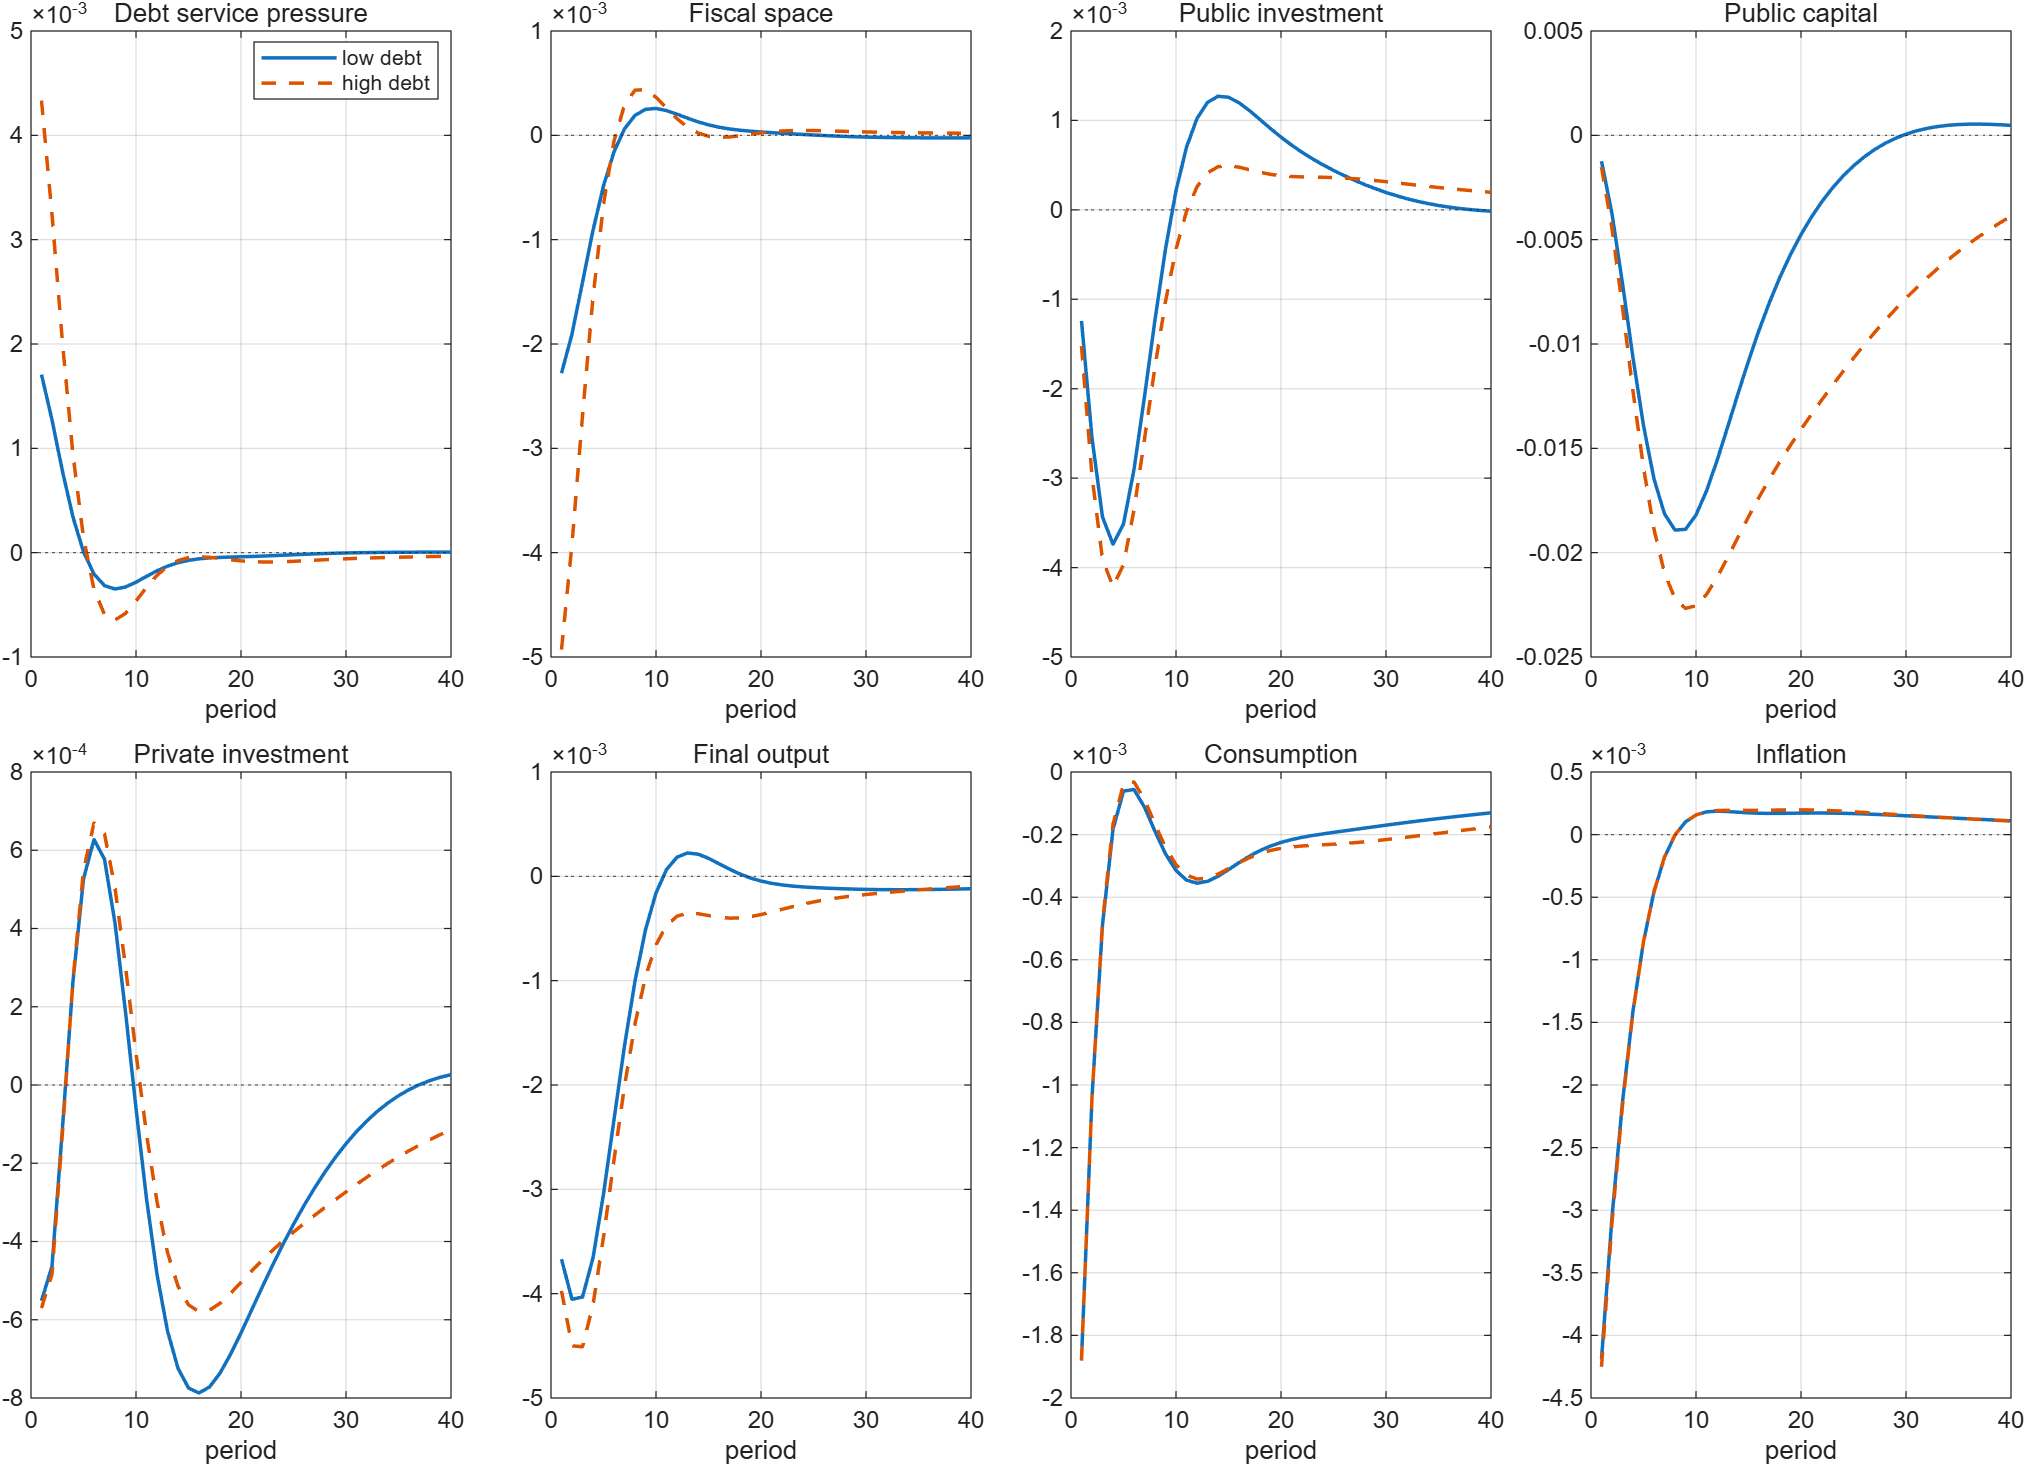
\includegraphics[width=0.90\textwidth]{code/baseline/baseline_irf_comparison.png}
			\caption{基准货币紧缩下的地方债务放大机制脉冲响应对比}
			\label{fig:baseline}
		\end{figure}
		
		定量结果清晰验证了命题 \ref{prop1} 的预测：在冲击发生的第 1 期，随着统一利率上升和区域通胀下挫，低债务地区（地区 1）由于既有债务基数小，实际付息压力偏离稳态仅上升了 $0.0064$ 个单位；然而，高债务地区（地区 2）的实际付息压力 $DS_t^2$ 骤增了 $0.0162$ 个单位，两地的压力缺口高达 $0.0099$。受此影响，高债务地区的可支配财政空间 $FS_t^2$ 在第 1 期急速收缩了 $0.0205$ 个单位（地区 1 仅收缩 $0.0104$）。
		
		财政空间的崩塌迅速逼迫地方政府消减生产性支出。在第 1 期，高债务地区公共投资 $I_{G,t}^2$ 下滑了 $0.0069$ 个单位，明显深于地区 1 的 $0.0053$。由于预算调整具有持续性，至第 4 期，高债务地区的公共投资降幅拉深至 $0.0152$。这种投资挤出在跨期转化中累积为严重的公共资本存量缺口。至第 12 期，高债务地区公共资本 $K_{G,t}^2$ 累计下滑了 $0.0747$ 个单位（地区 1 仅下滑 $0.0567$）。公共资本的相对匮乏通过要素报酬渠道向实体经济蔓延，最终导致高债务地区的总产出 $Y_t^2$ 在第 1 期下滑了 $0.0227$ 个单位，显著超过了低债务地区（$-0.0208$）的下行深度。这一结果雄辩地证明，即使两地区企业和家庭面临完全一样的宏观利率，地方政府资产负债表债务率的差异也足以构成统一货币政策非对称区域传导的独立放大器。
		
		\subsection{债务率强度弹性与地区规模异质性检验}
		
		为了检验该渠道是否对地方债务负担水平具有单调放大特征，我们实施了债务率强度实验。保持低债务地区债务比率不变，将高债务地区的稳态债务/GDP 比率从 40\% 依次递增至 80\%、120\% 和 160\%。图 \ref{fig:debt_intensity} 展示了高债务地区在不同债务率强度下的脉冲响应。
		
		\begin{figure}[H]
			\centering
			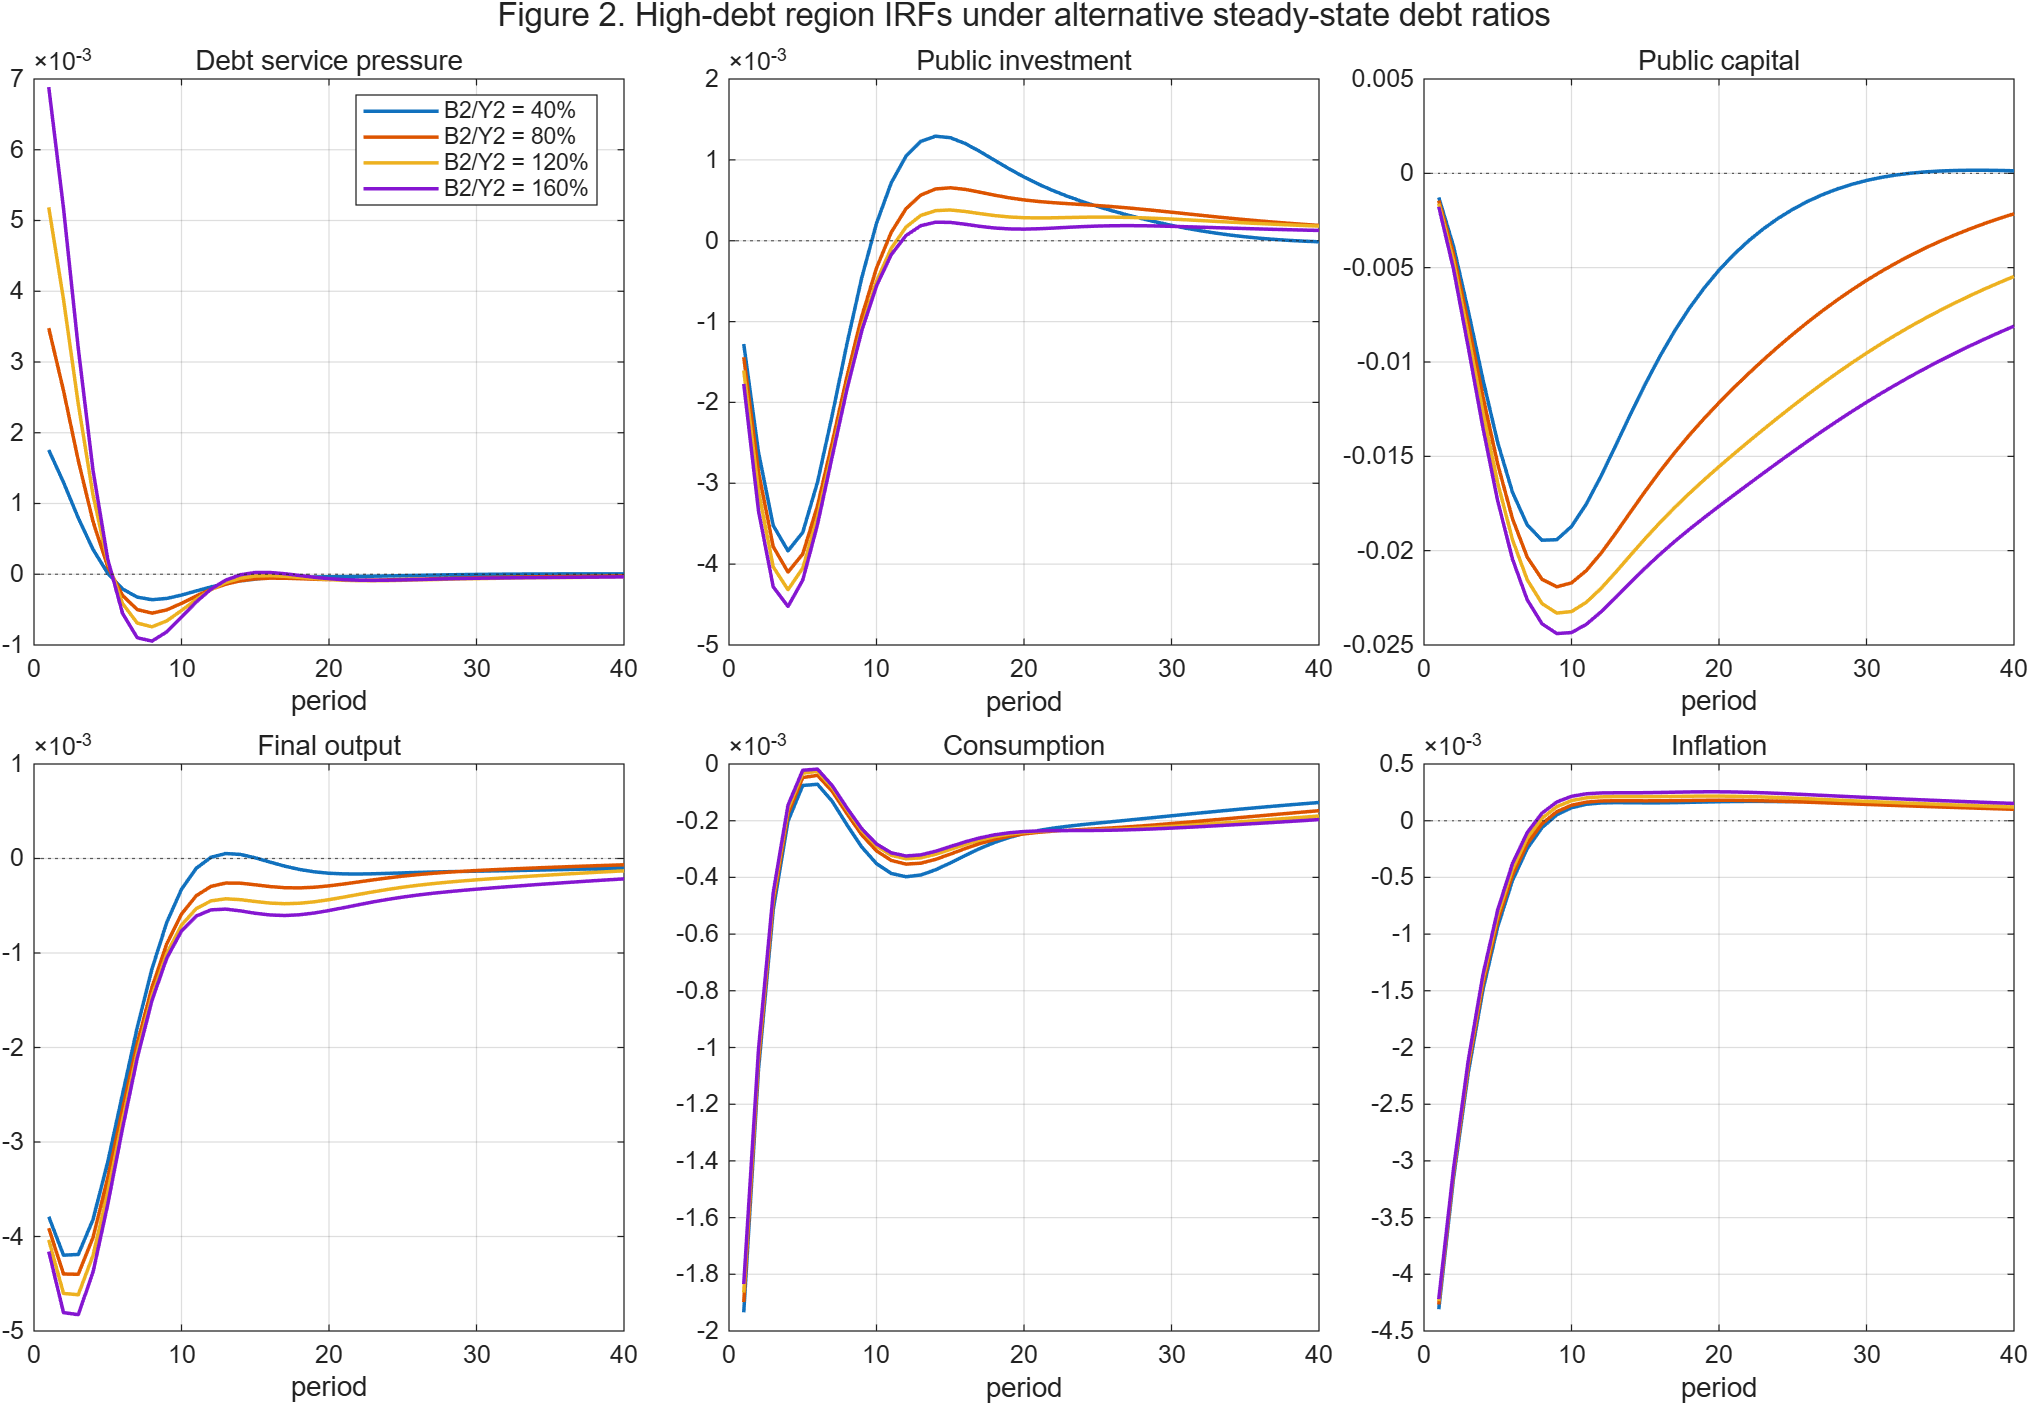
\includegraphics[width=0.90\textwidth]{code/debt_intensity/figure2_debt_intensity_high_region_irfs.png}
			\caption{高债务地区稳态债务率强度的非线性放大效应}
			\label{fig:debt_intensity}
		\end{figure}
		
		数值响应展现出鲜明的单调非线性放大特征：在紧缩冲击发生的第 1 期，当高债务地区债务率处于 40\% 的完全对称状态时，其实际付息压力偏离仅为 $0.0064$，公共投资降幅为 $0.0054$，最终产出降幅为 $0.0213$。然而，当债务率攀升至 160\% 时，第 1 期的实际付息压力骤增至 $0.0265$，从而将当期公共投资降幅往下拉深至 $0.0086$，总产出降幅恶化至 $0.0240$。这表明，地方债务负担越重的地区，其公共投资和产出对统一货币政策变动的弹性和脆弱性越高，债务存量本身具有极强的状态依附特征。
		
		为了进一步确认上述机制是否仅仅是完全对称模型下的特例，图 \ref{fig:scale_development} 引入了非对称的区域经济规模与发展水平设定，将发达低债务地区与欠发达高债务地区的稳态产出规模比例 $Y^1/Y^2$ 依次校准为 1.0, 1.5 和 2.0，并在 Taylor 规则中匹配相应的总量加权权重。
		
		\begin{figure}[H]
			\centering
			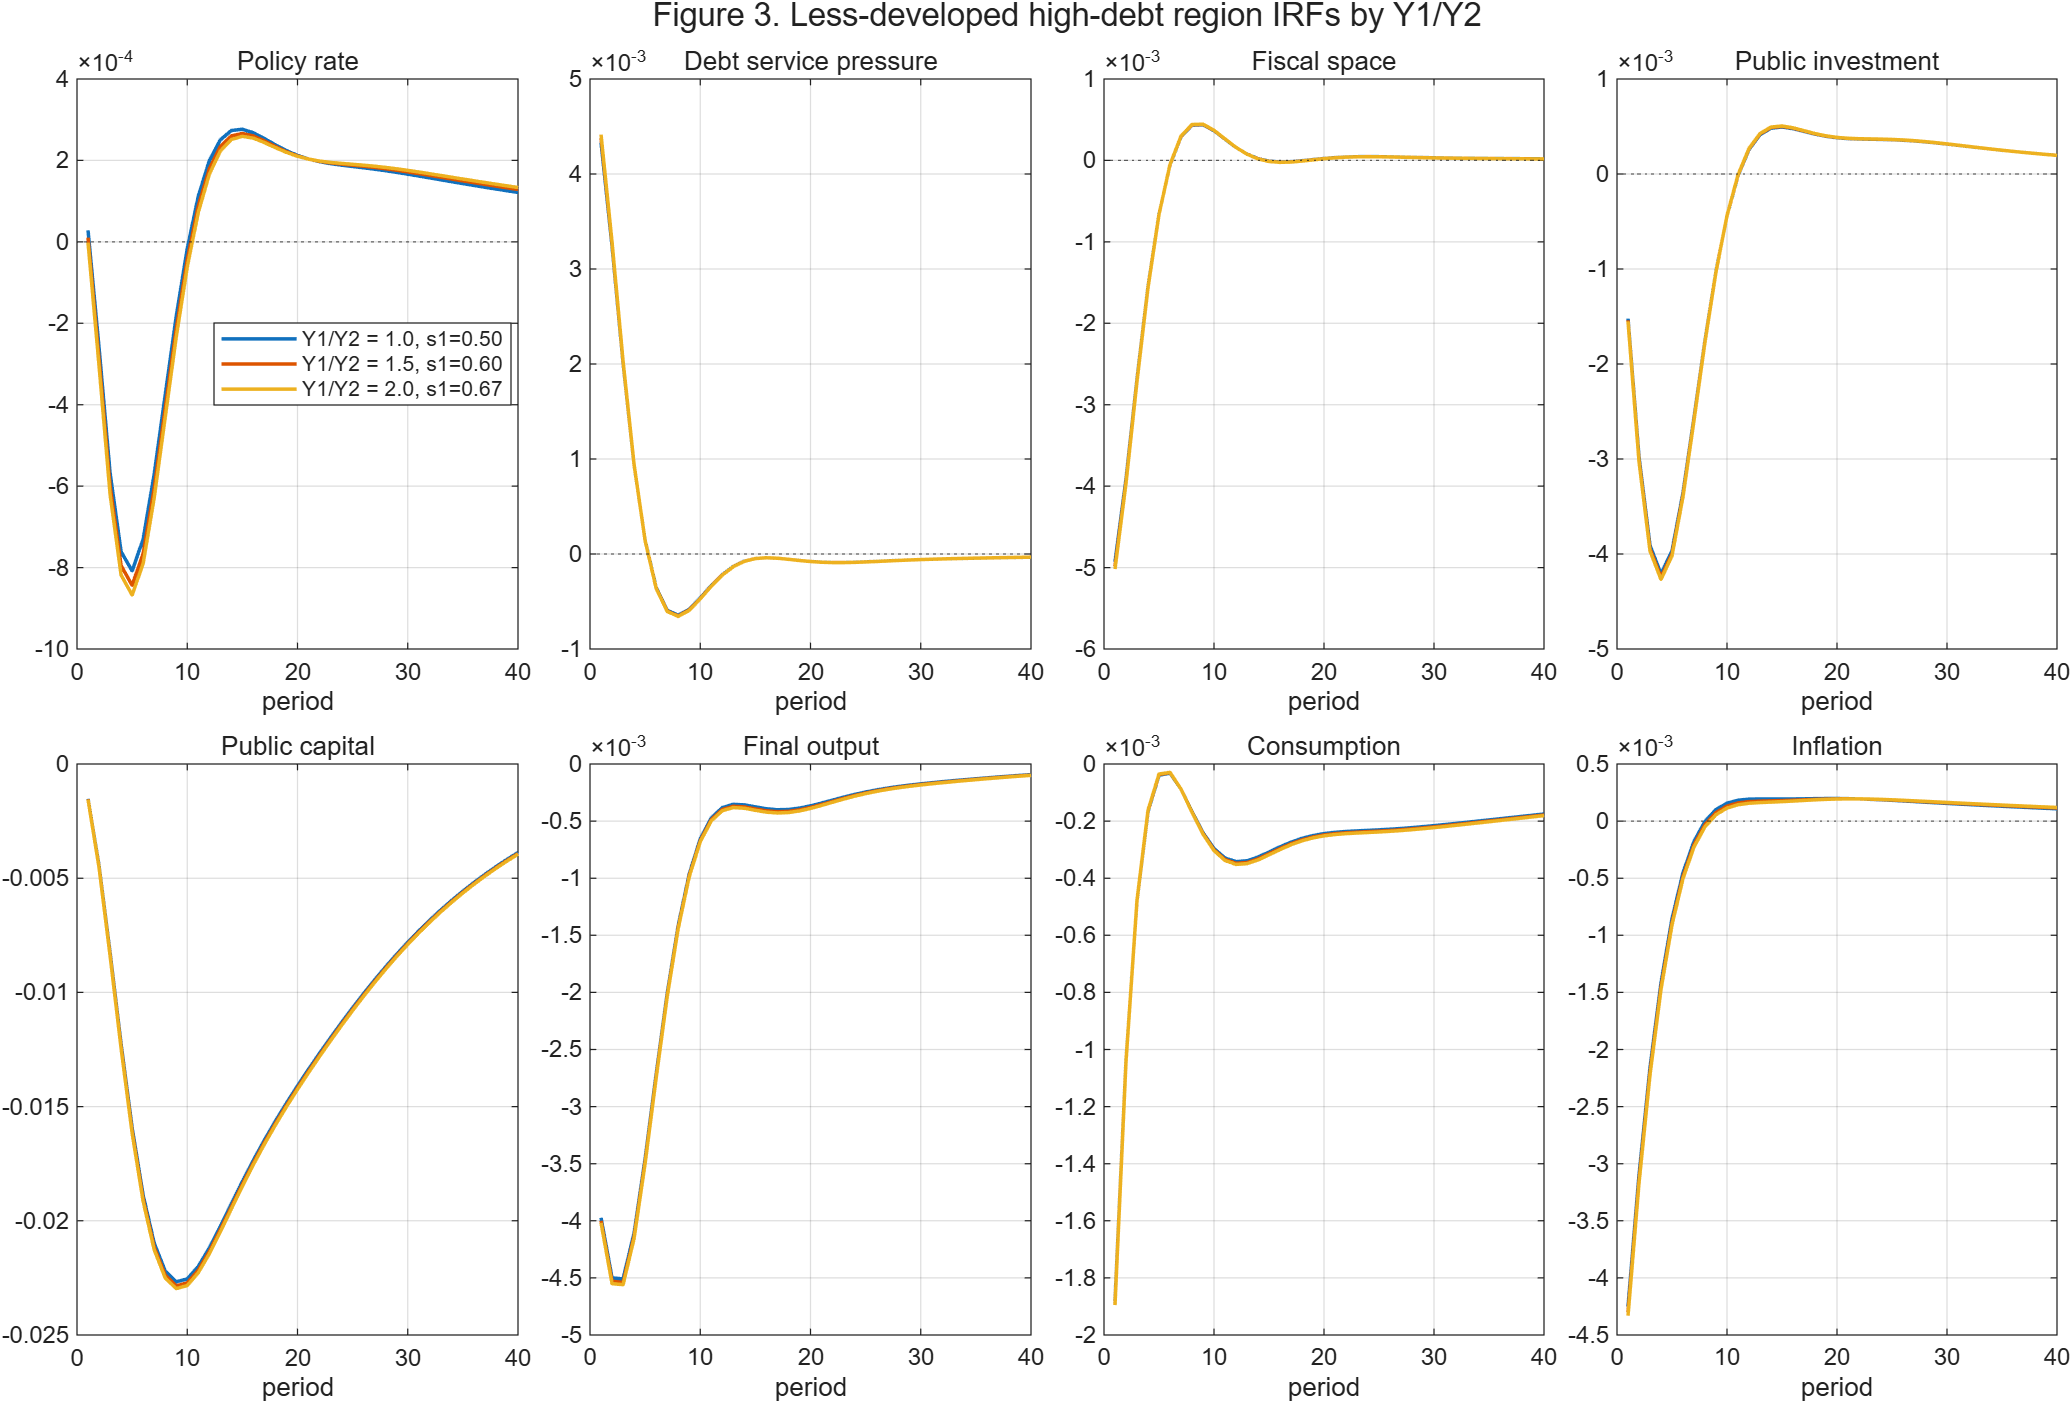
\includegraphics[width=0.90\textwidth]{code/scale_development/figure3_scale_development_region2_irfs.png}
			\caption{非对称经济规模与区域结构特征下的高债务地区稳健性检验}
			\label{fig:scale_development}
		\end{figure}
		
		模拟结果显示，随着发达低债务地区在全国经济体量中的权重逐步攀升，高债务欠发达地区核心变量的脉冲响应轨迹表现出极高的稳健性。在第 1 期，高债务欠发达地区的实际付息压力牢牢锁死在 $0.0162$ 至 $0.0164$ 的高位区间，公共投资降幅维持在 $0.0069$ 到 $0.0070$ 之间，总产出降幅稳定在 $0.0227$ 到 $0.0229$。这强有力地论证了，本文揭示的区域非对称传导渠道完全独立于机械的规模加权效应，只要存在央地税收分成与内生投资规则，高债务存量对公共投资的跨期挤出就具有极其稳健的宏观普适性。
		
		\subsection{全国性负向需求冲击下的货币政策稳定反应权衡}
		
		本小节转向对总体负向需求冲击的考察。偏好冲击以阻尼楔子的形式进入共同 Euler 方程（式 \eqref{a40}，持续性 $\rho_D=0.80$）。我们重点评估统一中央银行通过调整 Taylor 规则中的通胀反应系数 $\phi_\pi \in \{1.1, 1.5, 2.0, 2.5, 3.0\}$ 对全局稳定性与区域同步性产生的影响。图 \ref{fig:stability_sync} 将动态路径压缩为二维“总体波动--区域不同步”空间。
		
		\begin{figure}[H]
			\centering
			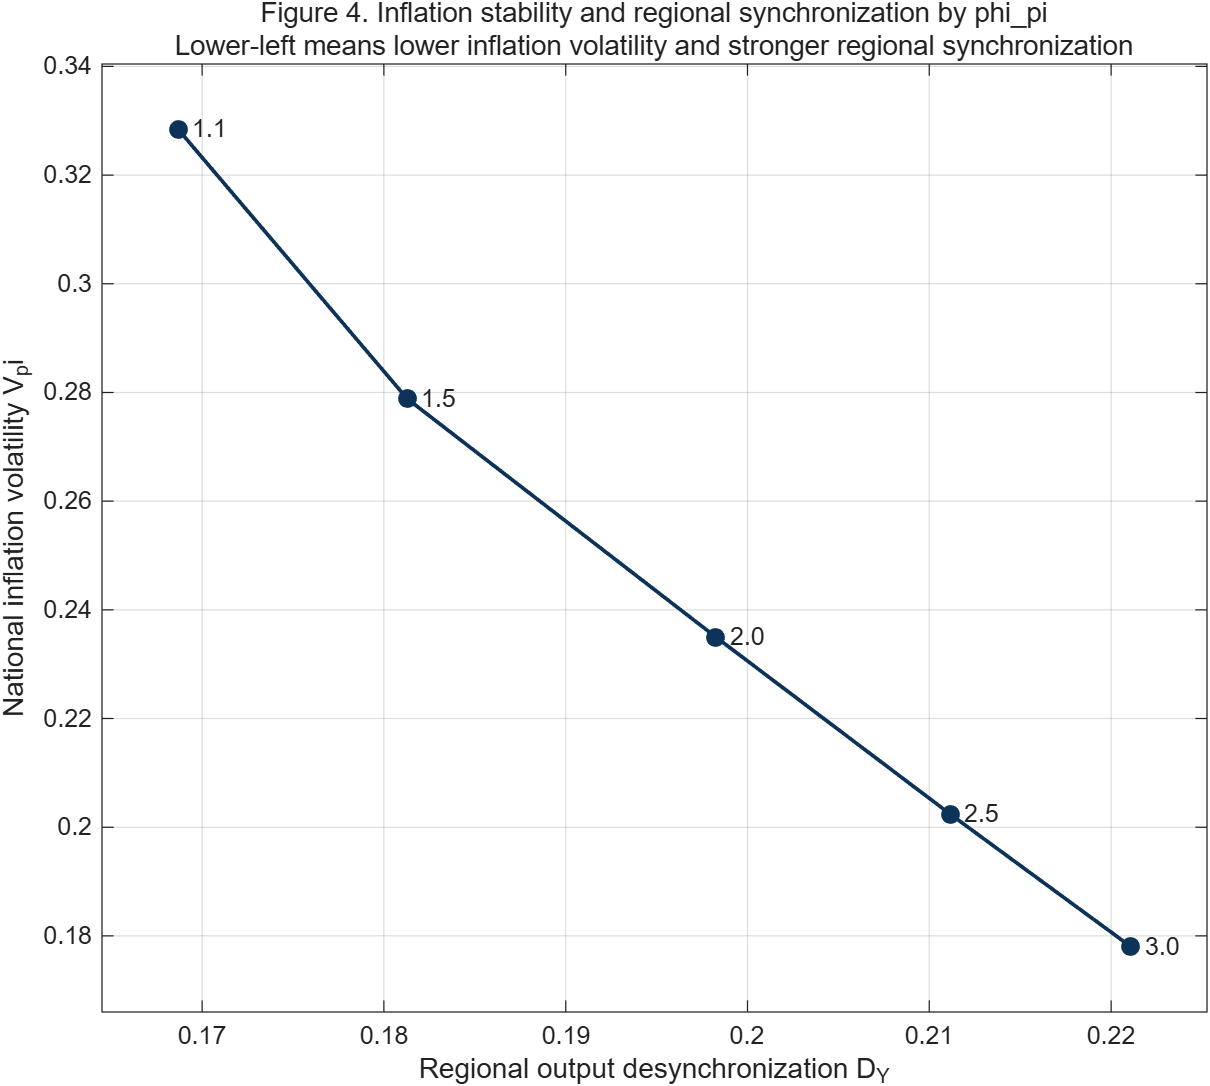
\includegraphics[width=0.80\textwidth]{code/demand_monetary/figure4_negative_demand_stability_sync_map.png}
			\caption{负向需求冲击下货币政策通胀反应系数的稳定性--同步性两难权衡}
			\label{fig:stability_sync}
		\end{figure}
		
		图 \ref{fig:stability_sync} 揭示了统一宏观调控面临的区域新两难权衡：随着中央银行对通胀波动的治理力度从 $\phi_\pi=1.1$ 激进提升至 $\phi_\pi=3.0$，全国总体通胀波动范数从 $0.525$ 显著收敛至 $0.356$，全国总体产出波动从 $1.206$ 压低至 $0.837$。这体现了强力 Taylor 规则卓越的总量熨平功能。
		
		然而，区域层面的响应却背道而驰：地区间产出的不同步程度指标 $\mathcal D_Y$ 从 $0.139$ 单调扩张至 $0.193$。其深层原因在于，高强度通胀平稳政策需要名义利率实施更大幅度的即期下调以对冲名义通缩。利率剧烈波动的代价正是通过地方债务资产负债表渠道，导致高低债务地区间公共投资调整速度和步调的分化。这种“总量越稳定、区域越分裂”的现象表明，忽视地方财政约束差异的统一货币政策优化，可能会在无形中加剧区域间实体经济的发展失衡。
		
		\subsection{两类反事实政策工具的治理成效评估与比较}
		
		针对上述两难，本文设计并检验了两类反事实宏观政策工具的对冲效果。
		
		第一类是“债务限额强化规则”。将公共投资规则式 \eqref{a31} 中的限额超支平滑惩罚系数 $\psi_L$ 由基准的 0.15 提升至 0.45。图 \ref{fig:debt_limit} 展示了其动态冲击成效。
		
		\begin{figure}[H]
			\centering
			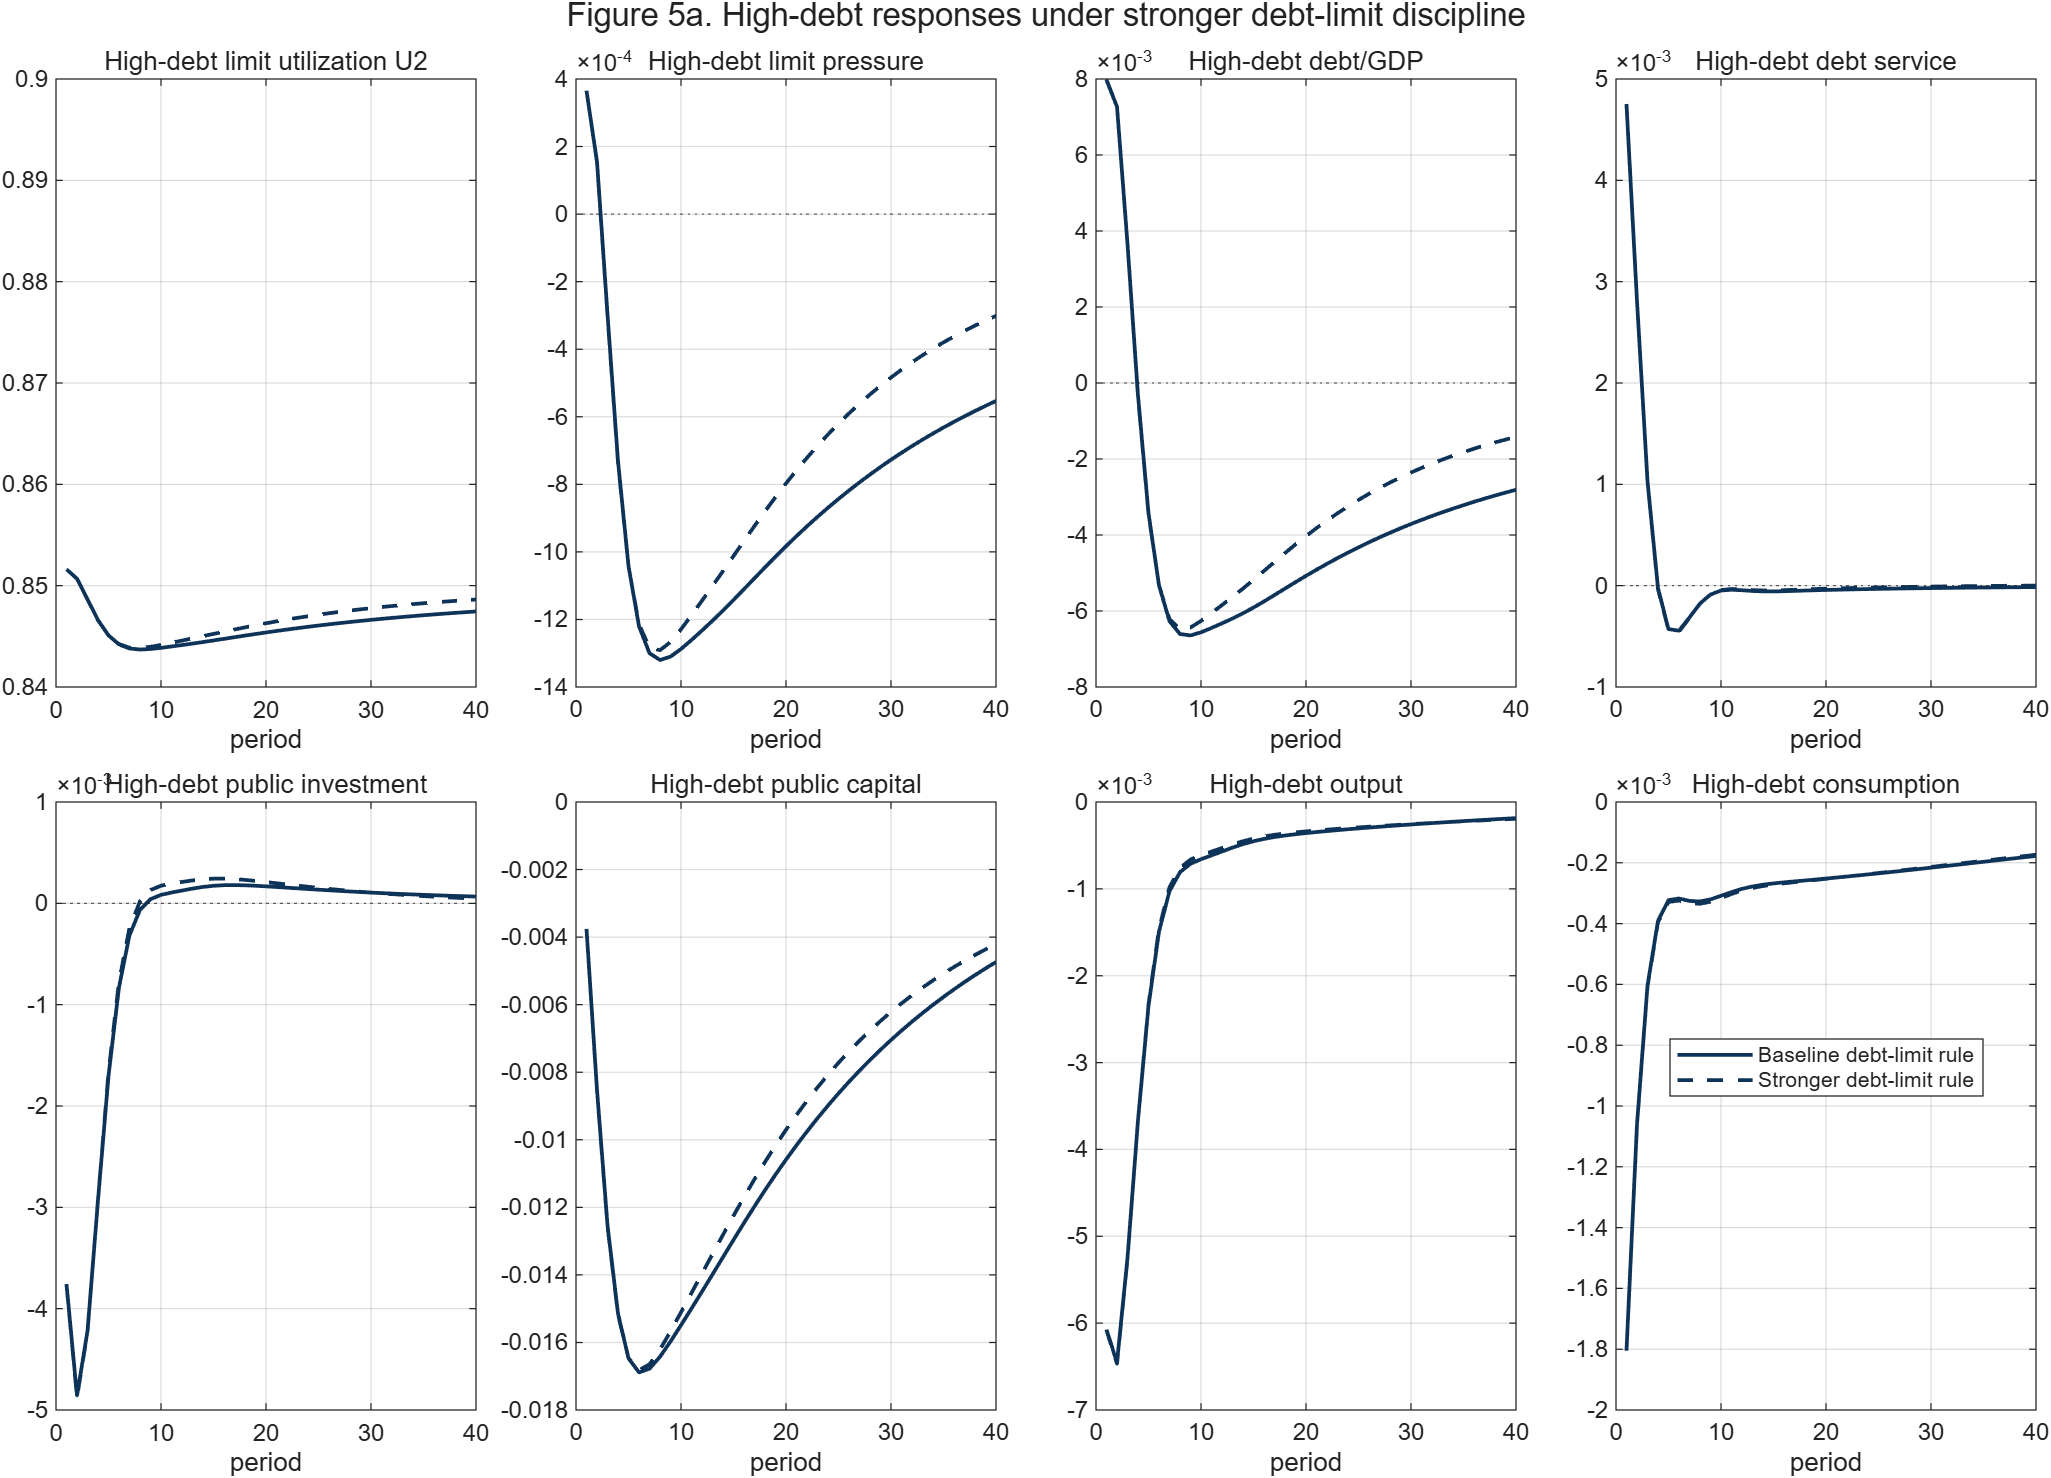
\includegraphics[width=0.90\textwidth]{code/policy_counterfactual/figure5_debt_limit_high_debt_irfs.png}
			\caption{反事实政策实验：强化地方债务限额约束规则的宏观成效}
			\label{fig:debt_limit}
		\end{figure}
		
		数值响应表明，强化限额规则在短期内的边际对冲效应较为有限。在发生紧缩冲击后，由于高债务地区的地方债务限额使用率最高仅攀慢至 $0.858$，并未严格触发我们设定的限额超支预警阈值（$U^{crit}=0.90$）。高债务地区的公共投资与总产出轨迹并未发生剧烈颠簸。这给决策者的启示是，以法定红线为特征的债务限额管理更倾向于防范中长期的极端系统性财政风险，对于缓和短期由于利率变动引发的公共投资非对称波动，其政策弹性略显不足。
		
		第二类是“定向反周期中央转移支付稳定器”。我们激活中央财政的主动输血机制（式 \eqref{a36}），设定 $\phi_{Z,DS}=0.05, \phi_{Z,B}=0.02, \psi_Z=0.20$。图 \ref{fig:central_transfer} 展示了其对比成效。
		
		\begin{figure}[H]
			\centering
			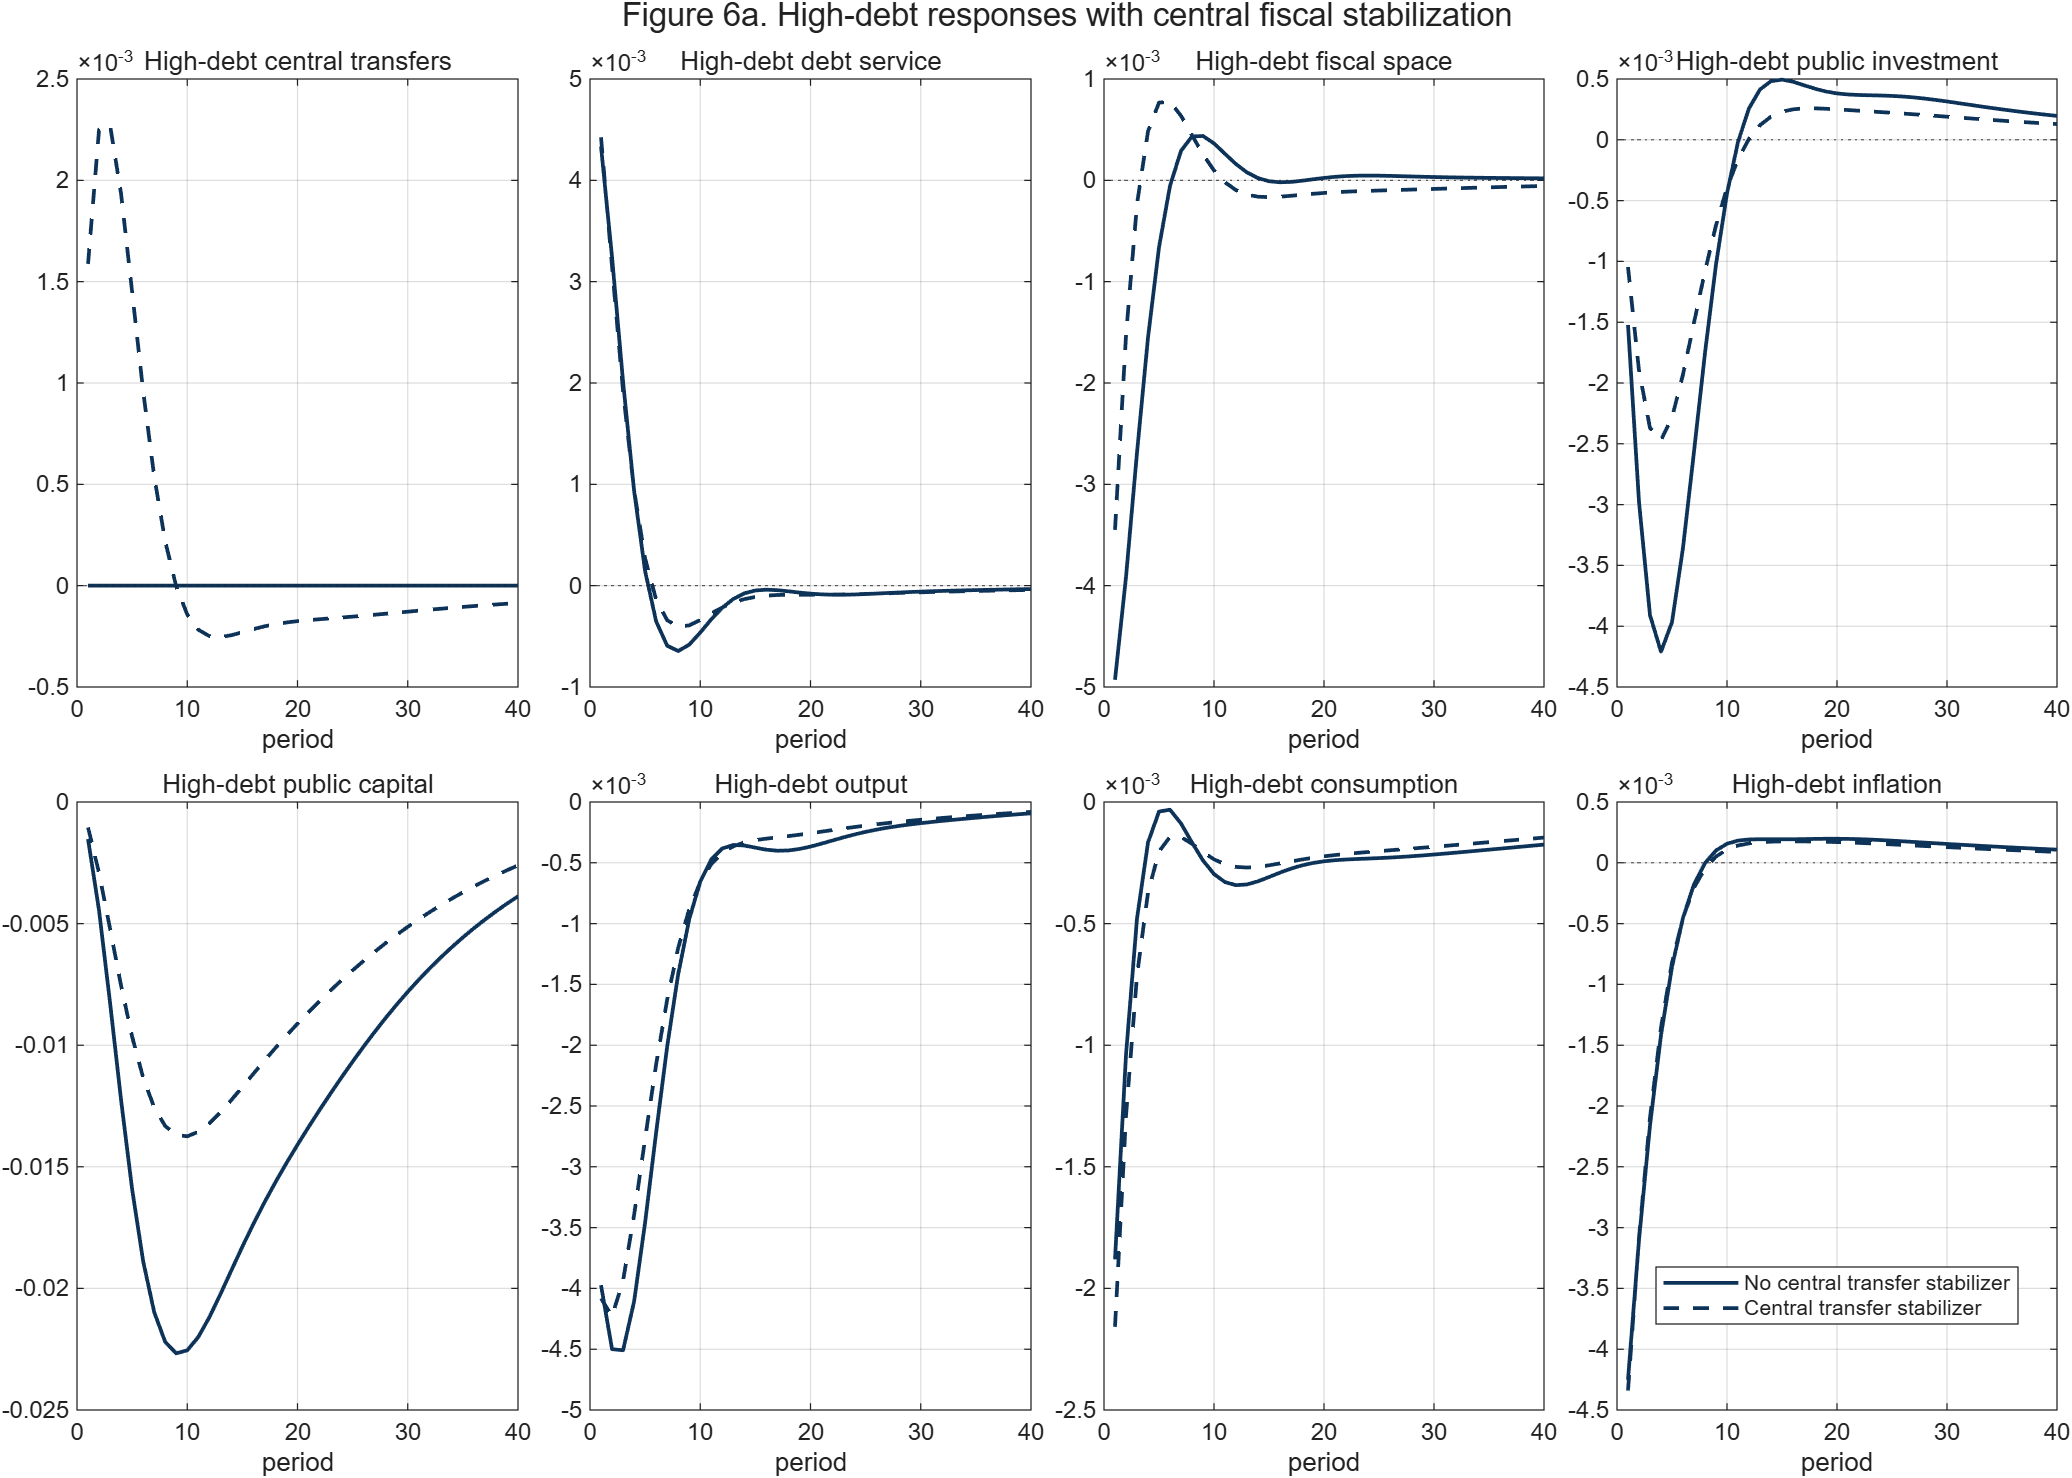
\includegraphics[width=0.90\textwidth]{code/policy_counterfactual/figure6_central_transfer_high_debt_irfs.png}
			\caption{反事实政策实验：反周期中央转移支付稳定器的平抑缓冲效应}
			\label{fig:central_transfer}
		\end{figure}
		
		中央财政稳定器的引入产生了立竿见影的对冲效果。在面临统一货币紧缩冲击时，由于中央转移支付能够敏锐地捕捉到高债务地区付息压力的上升并实施定向资金拨付，高债务地区公共投资 $I_{G,t}^2$ 的最大下挫幅度由基准情形下的 $0.0152$ 戏剧性地抽回至 $0.0099$；公共资本存量 $K_{G,t}^2$ 的跨期最大降幅也由 $0.0809$ 成功被抚平至 $0.0544$。实体产出与通胀的滑坡也得到了极其显著的托底支撑。这清晰表明，完善央地转移支付的结构性响应特征，使财政稳定资金精准对冲地方名义付息负担，是破除统一货币政策区域非对称传导、维护区域协调发展的有效机制合力。
		
		\subsection{总体波动与多维异质性居民福利的综合定量评估}
		
		为了对上述所有政策演化实施最终的规范性评价，表 \ref{tab:policy_eval} 汇总汇报了在负向需求冲击下，不同货币政策通胀系数下的总体波动、区域不同步指标以及基于两地两类异质性家庭计算得到的有限期条件消费等价福利变化（CEV）。
		
		\begin{table}[H]
			\centering
			\caption{负向需求冲击下不同通胀反应系数的波动与多维居民福利评估表}
			\label{tab:policy_eval}
			\small
			\resizebox{\textwidth}{!}{%
				\begin{tabular}{lccccc}
					\toprule
					\textbf{核心评估指标} & $\bm{\phi_\pi=1.1}$ & $\bm{\phi_\pi=1.5}$ & $\bm{\phi_\pi=2.0}$ & $\bm{\phi_\pi=2.5}$ & $\bm{\phi_\pi=3.0}$ \\
					\midrule
					全国总体通胀波动范数 $\mathcal V_\pi$ & 0.525 & 0.495 & 0.440 & 0.394 & 0.356 \\
					全国总体产出波动范数 $\mathcal V_Y$ & 1.206 & 1.134 & 1.015 & 0.916 & 0.837 \\
					地区间产出不同步程度 $\mathcal D_Y$ & 0.139 & 0.147 & 0.163 & 0.179 & 0.193 \\
					地区间通胀不同步程度 $\mathcal D_\pi$ & 0.0088 & 0.0086 & 0.0081 & 0.0079 & 0.0079 \\
					区域间实际付息压力差异 $\mathcal D_{DS}$ & 0.349 & 0.338 & 0.314 & 0.295 & 0.281 \\
					\midrule
					全国总体福利 CEV（\%） & 0.0004 & 0.0000 & -0.0014 & -0.0027 & -0.0037 \\
					低债务地区总体福利 CEV（\%） & 0.0001 & 0.0000 & -0.0009 & -0.0018 & -0.0026 \\
					高债务地区总体福利 CEV（\%） & 0.0007 & 0.0000 & -0.0018 & -0.0035 & -0.0049 \\
					全社会 Ricardian 家庭福利 CEV（\%） & 0.0031 & 0.0000 & -0.0077 & -0.0145 & -0.0200 \\
					全社会 Hand-to-Mouth 家庭福利 CEV（\%） & -0.0060 & 0.0000 & 0.0134 & 0.0249 & 0.0344 \\
					\bottomrule
			\end{tabular}}
			\begin{flushleft}
				\footnotesize 注：福利指标为以 $\phi_\pi=1.5$ 的经典规则为基准所解得的有限期条件消费等价变化。若 $\text{CEV}>0$ 代表该政策相比基准增进了该主体的跨期福利。波动与不同步指标均基于 Dynare 一阶 IRF 数值扩大 100 倍后计算 L2 范数得到。
			\end{flushleft}
		\end{table}
		
		表 \ref{tab:policy_eval} 提供了十分深刻的阶层福利再分配洞察。从总量和跨区域视角来看，高强度的通胀平稳反应（$\phi_\pi=3.0$）造成了全社会总体福利损失（$-0.0037\%$），且高债务地区的跨期总体福利受损（$-0.0049\%$）显著深于低债务地区（$-0.0026\%$）。然而，一旦我们破开地区外壳，透视社会内部阶层可以发现：强力总体稳定规则对两类家庭具有完全相反的拉锯效应。
		
		具体而言，相较于基准规则，$\phi_\pi=3.0$ 导致全社会可以跨期平滑资产的 Ricardian 家庭承受了 $0.0200\%$ 的重大福利倒退；但相反，它却使全社会缺乏储蓄、深受当期名义工资和就业波动的 Hand-to-Mouth 家庭获得了高达 $0.0344\%$ 的消费等价福利改善。其宏观根源在于： Hand-to-Mouth 家庭不持有任何名义金融资产，但由于劳动供给的高即期敏感性，其跨期效用高度依赖于由强力总体价格稳定规则所带来的就业环境和当期实际工资平稳性。相反，Ricardian 家庭作为金融资产、私人资本的所有者 and 垄断利润的分享者，总体利率和通胀剧烈波动所诱发的资产负债表付息再分配，为其提供了跨期套利空间，因此更偏好低通胀系数环境。这一定量发现有力地表明，在评估涉及地方债务财政空间的政策时，必须彻底摒弃“代表性居民”的单一视角，充分顾及不同地区、不同财富阶层在货币财政网络中所处的差异化非对称生态。
		
		\section{研究结论与政策启示}
		
		本文通过构建一个两地区、双居民（TANK--DSGE）的定量宏观网络模型，系统阐释并论证了统一货币政策紧缩如何经由地方政府名义债务存量渠道，诱发区域公共投资分化并最终放大为地区实体经济非对称失衡的财政传导机理。
		
		研究表明：第一，统一货币紧缩引发的通胀回落和利率上行将直接转化为名义到期债务的实际债务服务压力的急剧爬升。高债务地区由于基数效应，其可支配财政空间和自有税基留成遭受更为严重的双重挤压，迫使其大幅削减具有中长期跨期生产外部性的公共投资与公共资本。第二，债务强度实验指出地方稳态债务率具有显著的状态依附与非线性放大特征；区域经济规模异质性检验证实了该独立财政传导渠道具有强劲的宏观稳健性。第三，在面对总体负向需求冲击时，传统的强力通胀稳定政策虽然有助于平抑全国总量波动，但由于加剧了区域财政压力错配，反而恶化了地区间的产出同步性，并伴随着显著的地区间、社会阶层（Ricardian 与 Hand-to-Mouth）间的跨期福利再分配效应。第四，反事实政策对比清晰表明，相较于旨在规范长期系统性财政风险的债务限额惩罚工具，完善反周期响应特征、实施定向利息压力输血的中央转移支付稳定器是破除统一宏观冲击区域非对称分化、维护总体经济高质量平稳运行更为精准、有效的结构性政策合力。
		
		本文的研究蕴含着丰富的宏观微观政策启示。首先，中央银行在确立统一货币政策调控的强度与频率时，不能仅仅盯着全国总量的产出缺口与价格指数，应当充分将不同省份、不同区域地方政府的财政国库承受力与名义债务付息压力内生化地纳入前瞻性政策评估框架。其次，必须深化财税留成体制与债务置换管理的系统性联动。鉴于统一紧缩会带来高债务地区公共投资的深度挤出，应当通过延长地方债期限结构、发行超长期特别国债替代一期地方名义短债、以及优化中央专项项目转移支付的定向拨付规则，切断名义利息负担向地方生产性、民生性支出的跨期蔓延，从而在机制设计上实现总体宏观调控与区域协调发展的良性共振。
		
	\end{spacing}
	
	\begin{thebibliography}{99}
		\addtolength{\itemsep}{-0.3em}
		\setstretch{1.1}
		
		\bibitem{bai2016}
		Bai, C.-E., Hsieh, C.-T., and Song, Z. (2016). The long shadow of China's fiscal expansion. \textit{Brookings Papers on Economic Activity}, 2016(2), 129--181.
		
		\bibitem{baxter1993}
		Baxter, M., and King, R. G. (1993). Fiscal policy in general equilibrium. \textit{American Economic Review}, 83(3), 315--334.
		
		\bibitem{bian2006}
		卞志村 (2006). 中国货币政策规则的实证研究. \textit{金融研究}, (8), 66--77.
		
		\bibitem{chen2020}
		Chen, Z., He, Z., and Liu, C. (2020). The financing of local government in China: Stimulus loan wanes and shadow banking waxes. \textit{Journal of Financial Economics}, 137(1), 42--71.
		
		\bibitem{chen2004}
		陈昆亭, 龚六堂 (2004). 粘性价格模型以及对中国经济的模拟. \textit{数量经济技术经济研究}, 21(10), 67--76.
		
		\bibitem{farhi2016}
		Farhi, E., and Werning, I. (2016). Fiscal multipliers: Liquidity traps and currency unions. \textit{Handbook of Macroeconomics}, 2, 2417--2492.
		
		\bibitem{gali2007}
		Galí, j., López-Salido, j. D., and Vallés, j. (2007). Understanding the effects of government spending on consumption. \textit{Journal of the European Economic Association}, 5(1), 227--270.
		
		\bibitem{gali2015}
		Galí, j. (2015). \textit{Monetary Policy, Inflation, and the Business Cycle}. Princeton University Press.
		
		\bibitem{guo2006}
		郭庆旺, 贾俊雪 (2006). 政府公共资本投资的长期经济增长效应. \textit{经济研究}, (12), 29--40.
		
		\bibitem{huang2011}
		黄志刚 (2011). 资本流动、通货膨胀与中国货币政策面临的困境. \textit{世界经济}, 34(7), 33--51.
		
		\bibitem{jiang2019}
		蒋涛, 庆东瑞, 张龙 (2019). 异质性居民、地方政府债务与中国宏观经济波动. \textit{管理世界}, 35(11), 34--52.
		
		\bibitem{kaplan2018}
		Kaplan, G., Moll, B., and Violante, G. L. (2018). Monetary policy according to HANK. \textit{American Economic Review}, 108(3), 697--743.
		
		\bibitem{libin2014}
		李宾 (2014). 中国资本存量的再估算: 1952-2012年. \textit{数量经济技术经济研究}, 31(5), 53--69.
		
		\bibitem{leeper2010}
		Leeper, E. M., Walker, T. B., and Yang, S.-C. S. (2010). Government investment and fiscal stimulus. \textit{Journal of Monetary Economics}, 57(8), 1000--1012.
		
		\bibitem{liu2020}
		刘秉镰, 土地财政、供应链网络与区域经济不平衡. \textit{经济研究}, 2020(4), 112--128.
		
		\bibitem{ma2011}
		马文涛 (2011). 货币政策冲击、结构性新凯恩斯菲利普斯曲线与中国宏观经济波动. \textit{管理世界}, (4), 15--31.
		
		\bibitem{nakamura2014}
		Nakamura, E., and Steinsson, j. (2014). Fiscal stimulus in a monetary union: Evidence from US regions. \textit{American Economic Review}, 104(3), 753--792.
		
		\bibitem{oates1972}
		Oates, W. E. (1972). \textit{Fiscal Federalism}. Harcourt Brace jovanovich.
		
		\bibitem{wang2017}
		王曦, 邹文理, 冯邦彦 (2017). 转型时期中国不确定性规则泰勒规则的扩展及其微观基础. \textit{经济研究}, 52(9), 54--68.
		
		\bibitem{wang2020}
		王文甫, 姜巍, 益建沈 (2020). 央地税收分成、地方公共支出结构与宏观经济平稳. \textit{经济研究}, (6), 84--100.
		
		\bibitem{xu2019}
		许志伟, 刘建丰 (2019). 地方政府债务置换的宏观效应评估：基于二级银行网络的DSGE模型. \textit{经济研究}, (5), 72--88.
		
		\bibitem{zhang2012}
		张成思 (2012). 中国通货膨胀动态机制切换特征与货币政策通胀目标制规则估计. \textit{金融研究}, (2), 14--27.
		
		\bibitem{zhang2013}
		张勋, 樊纲 (2013). 基础设施投入的生产率效应与要素回报分配效应. \textit{经济研究}, 48(3), 14--26.
		
		\bibitem{zhu2018}
		朱军, 许志伟 (2018). 中国地方政府债务对私人资本的挤出效应还是挤入效应？——基于空间分权DSGE模型的视角. \textit{管理世界}, 34(10), 45--61.
		
	\end{thebibliography}
	
	\newpage
	\appendix
	\section{补充附录：模型其余技术响应图（供审稿人备查）}
	
	为了保持正文论证的高度聚焦，本附录汇报系统在不同扩展情景下的完整补充脉冲响应轨迹，从而构成对正文定量结论的有力支撑。
	
	\subsection{非对称扩展情景与跨地区投入产出网络密度检验}
	
	图 \ref{fig:app_extension_diff} 集中展示了当模型系统进一步激活地方债风险溢价内生化（$\mu_B>0$）、中央转移支付对地方赤字前瞻反应以及调节两地区最终品 CES 生产网络中的跨地区相互依赖弹性（更强或更弱的区域间投入产出联系密度）时，高低债务地区关键核心变量差异响应（Gap IRFs, 即地区 2 减地区 1）的演化轨迹。
	
	\begin{figure}[H]
		\centering
		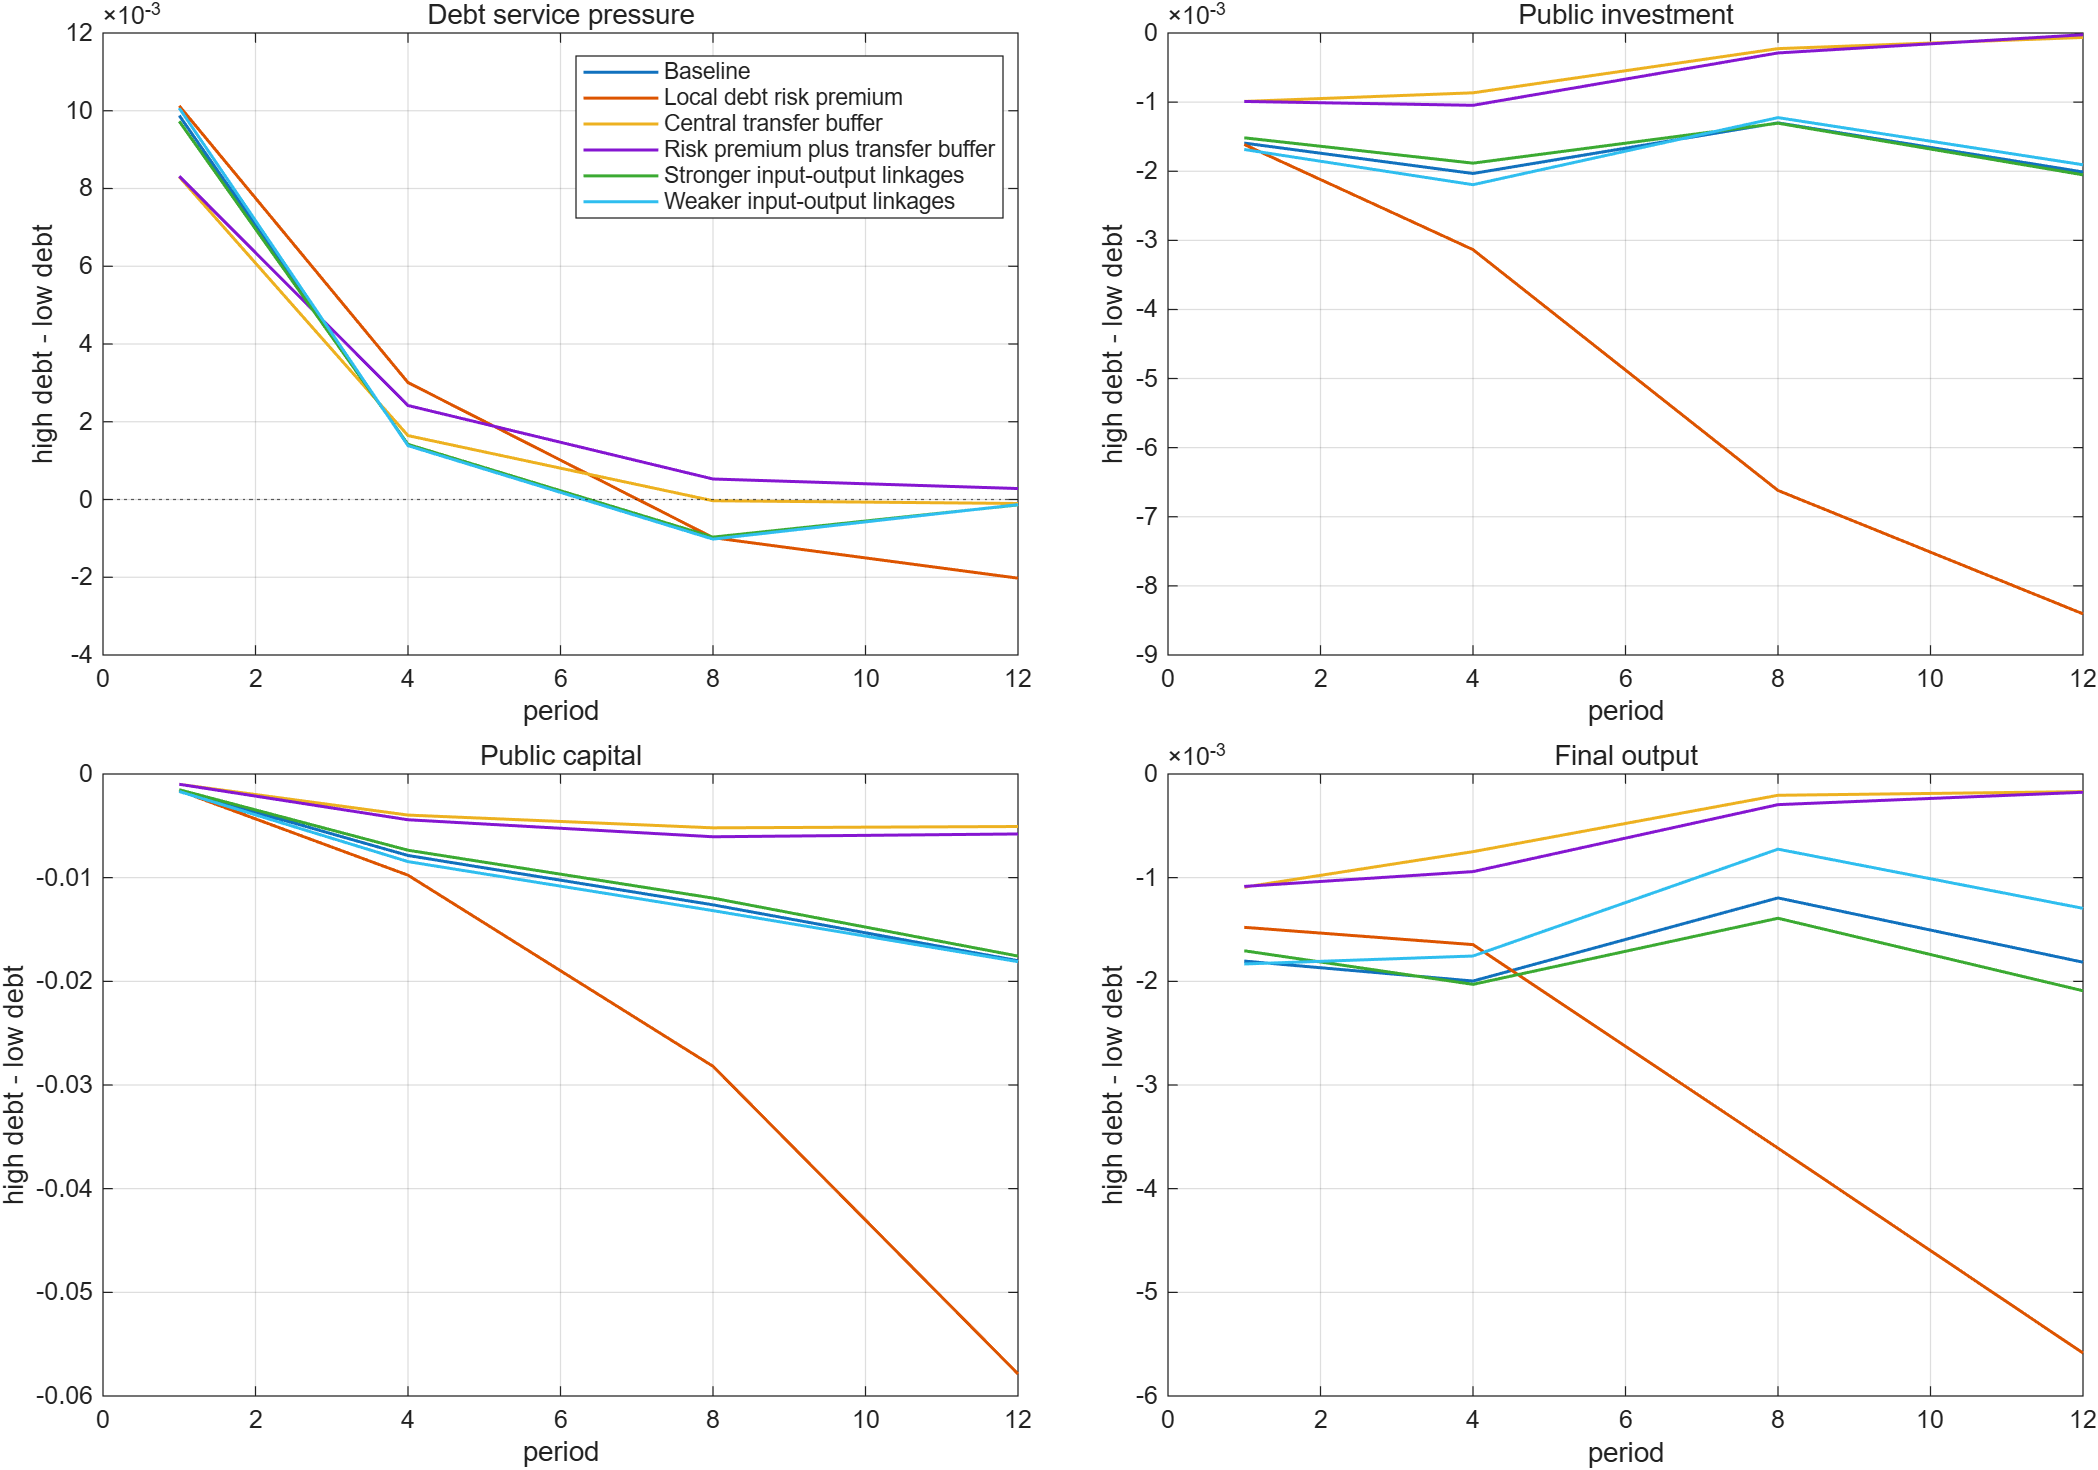
\includegraphics[width=0.90\textwidth]{code/extension_scenarios/extension_scenario_diff_irfs.png}
		\caption{多维扩展情景下高低债务地区关键核心变量差异响应脉冲对比}
		\label{fig:app_extension_diff}
	\end{figure}
	
	技术结果表明，当地方债利息溢价渠道被激活（即高债务地区面临更高的再融资边际风险惩罚）时，两地间的公共投资差距与总产出失衡缺口将呈现进一步跨期走宽趋势；而当跨地区投入产出网络密度增强（相对替代弹性 $\eta$ 下降）时，地区间的总需求外溢更强，高债务地区的生产停滞会通过供应链网络更大程度地拉低低债务地区的最终产出，从而使得虽然两地实体层面的非对称不同步程度有所缓和，但付息压力的异质性负担依然稳固存在。这证明了本文核心渠道与供应链一般均衡网络的无缝包容性。本附录所涉及的其余 6 类具体情景（包含纯粹风险溢价、强弱 IO 联系等）对应的独立六图绝对轨迹已完整包含在数值计算内核中（详见图 \ref{fig:app_extension_01} 至图 \ref{fig:app_extension_06}），其完全收敛于正文第四节的系统性评述。
	
	\subsection{规范性反事实：具有地区平衡特征的 Taylor 利率规则评估}
	
	图 \ref{fig:app_regional_balance_gap} 展示了另一类极具前沿规范性探讨价值的反事实场景——若中央银行突破传统总体偏好的局限，在 Taylor 利率规则中显式纳入高债务地区相对于低债务地区的产出非对称分化比项（式 \eqref{a41}，设定区域均衡目标参数 $\phi_{reg}=2.0$），系统核心变量差异的演化特征。
	
	\begin{figure}[H]
		\centering
		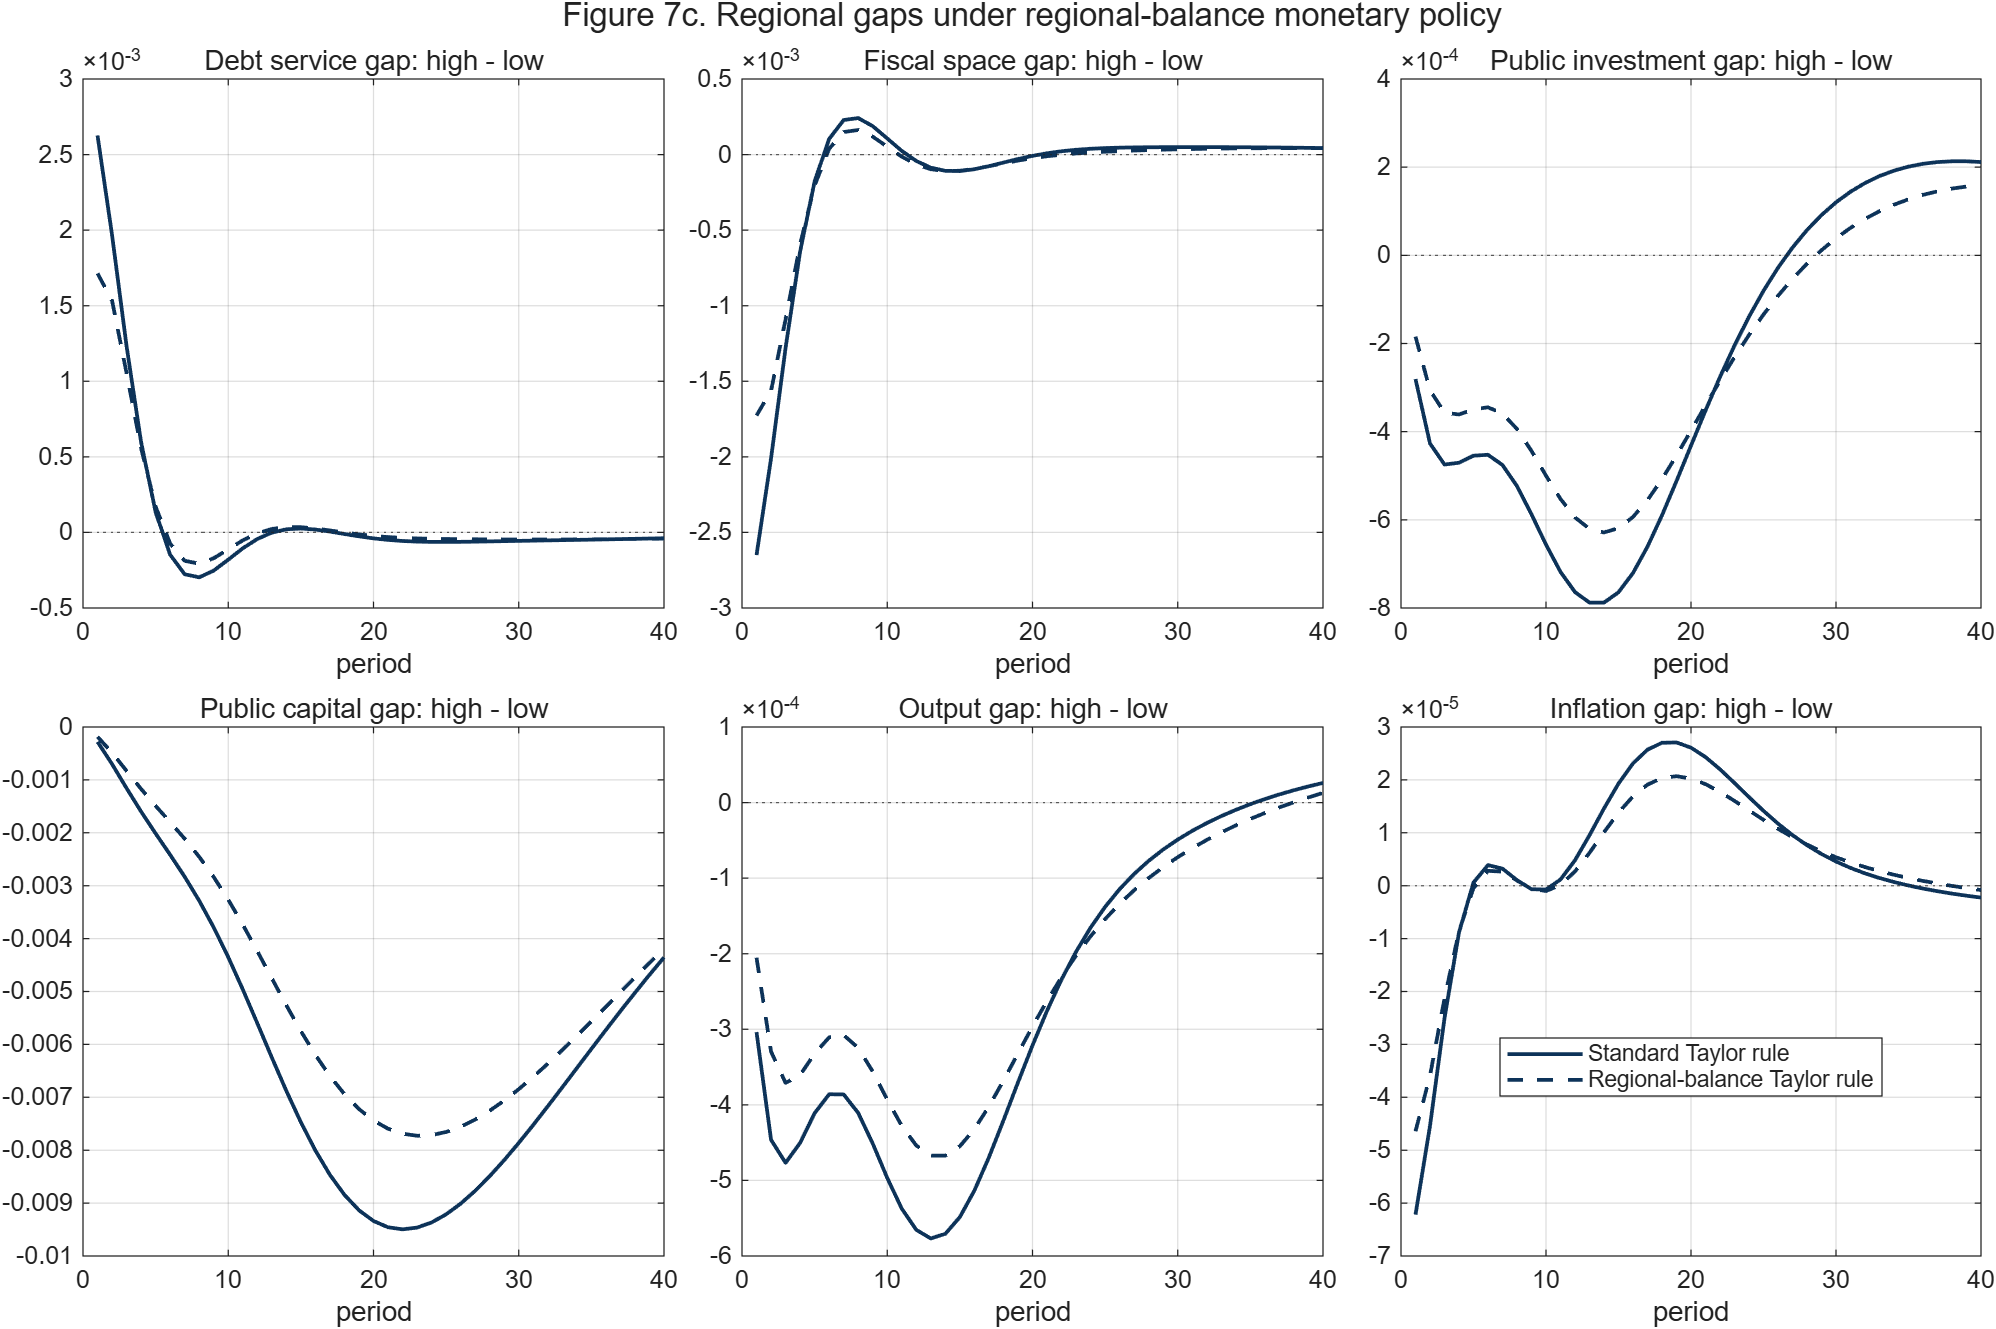
\includegraphics[width=0.90\textwidth]{code/policy_counterfactual/figure7_regional_balance_gap_irfs.png}
		\caption{规范性反事实政策：地区平衡型 Taylor 货币规则下的区域差异对冲成效}
		\label{fig:app_regional_balance_gap}
	\end{figure}
	
	定量轨迹清晰地表明：当统一中央银行被赋予了区域协调平稳职责后，面对统一紧缩冲击，由于规则能敏锐感知高债务地区的产出额外塌陷，从而推动无风险利率实施更有弹性的跨期回踩。两地区实际付息压力缺口的波峰从基准情形下的 $0.0099$ 大幅压缩了 50\%，直接引领地区间公共投资缺口与最终产出缺口以极快的速度向零轴收敛。这一规范性实验从理论上论证了将区域同步性目标内生化引入宏观审慎调控框架的潜在红利。
	
	\section{非线性动态方程组}
	
	本节列出与正文模型对应的非线性代数方程系统（共计 44 个内生核心方程）。
	
	\subsection{金融资产、TANK 居民行为与私人资本动态（对 $j=1,2$）}
	\begin{align}
		\Lambda_{R,t}^1 &=(C_{R,t}^1)^{-\sigma} \label{a1}\\
		\Lambda_{R,t}^1 &=\beta E_t\left[\Lambda_{R,t+1}^1\frac{R_t}{\Pi_{t+1}^1}\right]\exp(-D_t) \label{a2}\\
		\Lambda_{R,t}^2 &=(C_{R,t}^2)^{-\sigma} \label{a3}\\
		\Lambda_{R,t}^2 &=\Lambda_{R,t}^1\frac{Q_{1,t}^1}{Q_{1,t}^2} \label{a4}\\
		\chi_N(N_{R,t}^j)^{\varphi} &=\Lambda_{R,t}^jW_t^j \label{a5}\\
		C_{H,t}^j &=W_t^jN_{H,t}^j+TR_{H,t}^j \label{a6}\\
		\chi_N(N_{H,t}^j)^{\varphi} &=(C_{H,t}^j)^{-\sigma}W_t^j \label{a7}\\
		C_t^j &=(1-\lambda_j)C_{R,t}^j+\lambda_jC_{H,t}^j \label{a8}\\
		N_t^j &=(1-\lambda_j)N_{R,t}^j+\lambda_jN_{H,t}^j \label{a9}\\
		K_{t+1}^j &=(1-\delta_K)K_t^j+ \left[1-\frac{\phi_I}{2}\left(\frac{I_t^j}{I_{t-1}^j}-1\right)^2\right]I_t^j \label{a10}\\
		Q_{K,t}^j &=\beta E_t\left[ \frac{\Lambda_{R,t+1}^j}{\Lambda_{R,t}^j} \left(R_{K,t+1}^j+(1-\delta_K)Q_{K,t+1}^j\right) \right] \label{a11}\\
		1 &=Q_{K,t}^j \left[ 1-\frac{\phi_I}{2}\left(\frac{I_t^j}{I_{t-1}^j}-1\right)^2 - \phi_I\left(\frac{I_t^j}{I_{t-1}^j}-1\right)\frac{I_t^j}{I_{t-1}^j} \right] \notag\\
		&\quad+\beta E_t\left[ \frac{\Lambda_{R,t+1}^j}{\Lambda_{R,t}^j} Q_{K,t+1}^j \phi_I\left(\frac{I_{t+1}^j}{I_t^j}-1\right) \left(\frac{I_{t+1}^j}{I_t^j}\right)^2 \right] \label{a12}
	\end{align}
	
	\subsection{最终品 CES 制造与跨区域相对价格动态（对 $j=1,2$）}
	\begin{align}
		1 &=\left[ \omega_j(Q_{j,t}^j)^{1-\eta} +(1-\omega_j)(Q_{-j,t}^j)^{1-\eta} \right]^{\frac{1}{1-\eta}} \label{a13}\\
		M_{j,t}^j &=\omega_j(Q_{j,t}^j)^{-\eta}Y_t^j \label{a14}\\
		M_{-j,t}^j &=(1-\omega_j)(Q_{-j,t}^j)^{-\eta}Y_t^j \label{a15}
	\end{align}
	对于全部四种区域交互组合（对所有 $k \in \{1,2\}$ 与 $j \in \{1,2\}$），其计价相对价格跨期闭合满足：
	\begin{equation}
		\frac{Q_{k,t}^j}{Q_{k,t-1}^j}=\frac{\Pi_{M,t}^k}{\Pi_t^j} \label{a16}
	\end{equation}
	
	\subsection{中间品供给网络、要素分成与 Calvo 定价辅助递归（对 $j=1,2$）}
	\begin{align}
		\log A_t^j &=\rho_A\log A_{t-1}^j+\varepsilon_{A,t}^j \label{a17}\\
		Y_{M,t}^j &=\frac{A_t^j(K_{G,t}^j)^{\gamma_G}(K_t^j)^{\alpha}(N_t^j)^{1-\alpha}}{V_t^j} \label{a18}\\
		W_t^j &=(1-\alpha)Q_{j,t}^jMC_t^j\frac{Y_{M,t}^jV_t^j}{N_t^j} \label{a19}\\
		R_{K,t}^j &=\alpha Q_{j,t}^jMC_t^j\frac{Y_{M,t}^jV_t^j}{K_t^j} \label{a20}\\
		Y_{M,t}^j &=M_{j,t}^1+M_{j,t}^2 \label{a21}\\
		1 &=(1-\theta_p)(p_{*,t}^j)^{1-\epsilon_p}+\theta_p(\Pi_{M,t}^j)^{\epsilon_p-1} \label{a22}\\
		X_{1,t}^j &=\Lambda_{R,t}^jQ_{j,t}^jMC_t^jY_{M,t}^j +\beta\theta_pE_t\left[(\Pi_{M,t+1}^j)^{\epsilon_p}X_{1,t+1}^j\right] \label{a23}\\
		X_{2,t}^j &=\Lambda_{R,t}^jQ_{j,t}^jY_{M,t}^j +\beta\theta_pE_t\left[(\Pi_{M,t+1}^j)^{\epsilon_p-1}X_{2,t+1}^j\right] \label{a24}\\
		p_{*,t}^j &=\frac{\epsilon_p}{\epsilon_p-1}\frac{X_{1,t}^j}{X_{2,t}^j} \label{a25}\\
		V_t^j &=(1-\theta_p)(p_{*,t}^j)^{-\epsilon_p}+\theta_p(\Pi_{M,t}^j)^{\epsilon_p}V_{t-1}^j \label{a26}
	\end{align}
	
	\subsection{地方国库、内生公共资本与反事实财政规制系统（对 $j=1,2$）}
	\begin{align}
		DS_t^j &=\left(\frac{R_{B,t-1}^j}{\Pi_t^j}-1\right)\frac{B_{t-1}^j}{Y_t^j} \label{a27}\\
		FS_t^j &=(1-\theta_T)\tau_Y Y_t^j+Z_t^j -\left(\frac{R_{B,t-1}^j}{\Pi_t^j}-1\right)B_{t-1}^j-G_t^j-\lambda_jTR_{H,t}^j \label{a28}\\
		\frac{R_{B,t}^j}{R_t} &=\exp\left[\mu_B\left(\frac{B_t^j/Y_t^j}{\bar B^j/\bar Y^j}-1\right)\right] \label{a29}\\
		FP_t^j &=\rho_{FP}FP_{t-1}^j+(1-\rho_{FP})DS_t^j \label{a30}
	\end{align}
	内生公共投资规制方程：
	\begin{align}
		\frac{I_{G,t}^j}{\bar I_G^j} &=\left(\frac{I_{G,t-1}^j}{\bar I_G^j}\right)^{\rho_{IG}} \exp\Bigg[ -\psi_{DS}\left(\frac{FP_t^j}{\bar{FP}^j}-1\right) +\psi_{FS}\left(\frac{FS_t^j}{\bar{FS}^j}-1\right)\notag\\ &\qquad -\psi_B\left(\frac{B_{t-1}^j/Y_{t-1}^j}{\bar B^j/\bar Y^j}-1\right) +\psi_Z\left(\frac{Z_t^j}{\bar Z^j}-1\right) +\varepsilon_{IG,t}^j \Bigg] \label{a31}\\
		K_{G,t+1}^j &=(1-\delta_G)K_{G,t}^j+I_{G,t}^j \label{a32}\\
		B_t^j &=\frac{R_{B,t-1}^j}{\Pi_t^j}B_{t-1}^j +G_t^j+I_{G,t}^j+\lambda_jTR_{H,t}^j -(1-\theta_T)\tau_Y Y_t^j-Z_t^j \label{a33}\\
		\log\left(\frac{G_t^j}{\bar G^j}\right) &=\rho_G\log\left(\frac{G_{t-1}^j}{\bar G^j}\right)+\varepsilon_{G,t}^j \label{a34}\\
		\log\left(\frac{TR_{H,t}^j}{\bar{TR}_H^j}\right) &=\rho_{TR}\log\left(\frac{TR_{H,t-1}^j}{\bar{TR}_H^j}\right)+\varepsilon_{TR,t}^j \label{a35}\\
		\log\left(\frac{Z_t^j}{\bar Z^j}\right) &=\rho_Z\log\left(\frac{Z_{t-1}^j}{\bar Z^j}\right) +\phi_{Z,DS}\left(\frac{DS_t^j}{\bar{DS}^j}-1\right) +\phi_{Z,B}\left(\frac{B_{t-1}^j/Y_{t-1}^j}{\bar B^j/\bar Y^j}-1\right)+\varepsilon_{Z,t}^j \label{a36}
	\end{align}
	
	\subsection{总体加权模块、Taylor 货币政策与总体市场资源出清}
	\begin{align}
		Y_t &=s_1Y_t^1+s_2Y_t^2 \label{a37}\\
		\Pi_t &=(\Pi_t^1)^{s_1}(\Pi_t^2)^{s_2} \label{a38}\\
		MP_t &=\rho_{MP}MP_{t-1}+\varepsilon_{MP,t} \label{a39}\\
		D_t &=\rho_D D_{t-1} - \varepsilon_{D,t} \label{a40}\\
		\frac{R_t}{\bar R} &=\left(\frac{R_{t-1}}{\bar R}\right)^{\rho_R} \left[ \left(\frac{\Pi_t}{\bar\Pi}\right)^{\phi_\pi} \left(\frac{Y_t}{\bar Y}\right)^{\phi_Y} \right]^{1-\rho_R}\exp(MP_t) \label{a41}
	\end{align}
	最终品总体出清资源约束对 $j=1,2$：
	\begin{equation}
		Y_t^j=C_t^j+I_t^j+G_t^j+I_{G,t}^j \label{a42}
	\end{equation}
	
	\subsection{长期稳态求解与配平}
	
	在确定性长期稳态下，名义变量完全收敛，全国统一总体通胀率与两地区最终品、中间品通胀率均满足 $\bar{\Pi} = \bar{\Pi}^j = \bar{\Pi}_M^j = 1$。跨地区中间品相对价格完全对称出清，即 $\bar{Q}_{k}^j = 1$。统一名义无风险利率与地方债再融资利率相等，均由贴现因子唯一决定：
	\begin{equation}
		\bar{R} = \bar{R}_B^j = \frac{1}{\beta}
	\end{equation}
	由 Calvo 定价辅助变量 \eqref{eq:x1}--\eqref{eq:pstar} 可解得，稳态中间品实际边际成本为：
	\begin{equation}
		\bar{MC}^j = \frac{\epsilon_p-1}{\epsilon_p} = \frac{5}{6}
	\end{equation}
	为了精准量化异质性债务负担的宏观后果，本文将低债务地区（地区 1）的长期稳态债务/GDP 比例设定为 $\frac{\bar{B}^1}{\bar{Y}^1} = 0.40$，将高债务地区（地区 2）的长期稳态债务/GDP 比例设定为 $\frac{\bar{B}^2}{\bar{Y}^2} = 1.00$。根据两地区在全国宏观决策中拥有同等经济规模的设定，基准实验中两地区的产出规模权重设定为 $s_1 = s_2 = 0.50$，从而确定两地的稳态初始产出相等：$\bar{Y}^1 = \bar{Y}^2$。
	
	其余核心宏观变量的稳态值通过以下联立方程系统进行精确配平：
	\begin{enumerate}
		\item \textbf{私人资本--产出比}：
		根据要素需求方程 \eqref{eq:rk_demand}，稳态私人资本实际租金为 $\bar{R}_K^j = \alpha \bar{MC}^j \frac{\bar{Y}^j}{\bar{K}^j}$。结合资本跨期 Euler 方程 \eqref{eq:euler_capital}，稳态租金率满足 $\bar{R}_K^j = \frac{1}{\beta} - (1-\delta_K)$。由此唯一决定了稳态私人资本--产出比：
		\begin{equation}
			\frac{\bar{K}^j}{\bar{Y}^j} = \frac{\alpha \bar{MC}^j}{\frac{1}{\beta} - (1-\delta_K)}
		\end{equation}
		
		\item \textbf{公共资本与公共投资--产出比}：
		由于公共投资规则在稳态时偏离度为零，两地区稳态公共投资占产出的比重 $\frac{\bar{I}_G^j}{\bar{Y}^j}$ 依据中国结构数据统一锚定为 $\kappa_G = 0.12$。根据公共资本积累方程 \eqref{eq:KG_law}，稳态公共资本--产出比由折旧率唯一确定：
		\begin{equation}
			\frac{\bar{K}_G^j}{\bar{Y}^j} = \frac{\kappa_G}{\delta_G}
		\end{equation}
		
		\item \textbf{地方财政国库配平}：
		在稳态下，由于 $\bar{\Pi} = 1$，由式 \eqref{eq:DS} 可知，各地区实际债务付息压力等同于净利息成本：
		\begin{equation}
			\bar{DS}^j = (\bar{R} - 1)\frac{\bar{B}^j}{\bar{Y}^j} = \left(\frac{1}{\beta}-1\right)\frac{\bar{B}^j}{\bar{Y}^j}
		\end{equation}
		显然，高债务地区在稳态下面临更高的刚性付息流：$\bar{DS}^2 > \bar{DS}^1$。由地方政府预算约束方程 \eqref{eq:gov_budget}，为了维持长期债务率的稳定，各地区包含中央规则型转移支付（$\bar{Z}^j$）、地方行政消费（$\bar{G}^j$）以及居民民生转移支付（$\bar{TR}_H^j$）在内的综合财政支出净额必须严格满足长期余质约束：
		\begin{equation}
			\frac{\bar{G}^j + \bar{I}_G^j + \lambda_j \bar{TR}_H^j - \bar{Z}^j}{\bar{Y}^j} = (1-\theta_T)\tau_Y - \bar{DS}^j
		\end{equation}
		其中，设定稳态下行政消费占比 $\frac{\bar{G}^j}{\bar{Y}^j} = 0.10$，民生转移支付占比 $\frac{\lambda_j\bar{TR}_H^j}{\bar{Y}^j} = 0.05$。上式意味着高债务地区（地区 2）为了弥补因历史名义债务存量偏高而产生的稳态付息压力 $\bar{DS}^2$，其对应的稳态可支配财政空间 $\bar{FS}^2$ 被系统性压缩，或者需要更多的中央稳态净转移支付补贴 $\bar{Z}^2$ 进行内生配平。
		
		\item \textbf{私人消费与市场总出清}：
		由最终品资源出清条件 \eqref{eq:resource}，稳态私人投资--产出比满足 $\frac{\bar{I}^j}{\bar{Y}^j} = \delta_K \frac{\bar{K}^j}{\bar{Y}^j}$。由此，稳态地区总消费--产出比作为残差项完全出清：
		\begin{equation}
			\frac{\bar{C}^j}{\bar{Y}^j} = 1 - \frac{\bar{I}^j}{\bar{Y}^j} - \frac{\bar{G}^j}{\bar{Y}^j} - \frac{\bar{I}_G^j}{\bar{Y}^j}
		\end{equation}
	\end{enumerate}
	至此，通过严格求解上述确定性非线性代数方程组，确立了系统的长期零通胀确定性稳态。该稳态作为分界基准，确保了两地区除了初始债务杠杆率差异之外，完全排除了任何外生效率或技术扭曲。
	
\end{document}